\documentclass[a4paper,12pt]{article}
\usepackage[a4paper,top=1.3cm,bottom=2cm,left=1.5cm,right=1.5cm,marginparwidth=0.75cm]{geometry}

% Пакеты
\usepackage{mathtext} 
\usepackage{setspace}
\usepackage{tabularx}
\usepackage{cmap}
\usepackage{longtable}
\usepackage{icomma}
\usepackage{euscript}
\usepackage{float}
\usepackage{cutwin}
\usepackage{mathrsfs}
\usepackage{adjustbox}
\usepackage{dashbox}
\usepackage[normalem]{ulem}
\usepackage[T2A]{fontenc}			
\usepackage[utf8]{inputenc}                 %!  закрепляет кодировку utf8
\usepackage[english,russian]{babel}         %!  подключает русский и английский
%математические шрифты:
\usepackage{amsmath,amsfonts,amssymb,amsthm,mathrsfs,mathtools} 
\usepackage[colorlinks, linkcolor = purple]{hyperref}      %!  оглавление для панели навигации по PDF-документу + гиперссылки
\usepackage{xcolor}                         %!  добавляет цвета
\usepackage{enumitem}                       %!  задание макета перечня.
\usepackage{xpatch}                         %?  работа с renewcommand и макросами              
\usepackage{cancel}                         %   зачёкивания текста (!!!) для slash-нотации использовать \usepackage{slashed}!!
\usepackage{upgreek}                        %   заглавные греческие буквы
\usepackage{lipsum}                         %?  для вставки кучи текста при форматировании
\usepackage[version=4]{mhchem}              %   химические формулы
\usepackage{multirow}                       %   объединение строк в матрицах
\usepackage{stackengine}                    %   stack символов
\usepackage{tikz}                           %!  рисунки
\usetikzlibrary{positioning}                %?  библиотека для тикза 
\usepackage{titletoc}                       %!  форматирование содержания и заголовков
\usepackage{titlesec}                       %!  форматирование содержания и заголовков
\usepackage{wrapfig}                        %   обтекание таблиц и рисунков
\usepackage{chngcntr}                       %!  для setcounter
\usepackage{fancyhdr}                       %!  для колонтитулов
\usepackage{makecell}                       %?  матрицы с разными выравниваниями и т.п
\usepackage{indentfirst}                    %   добавить indent перед первым 
\usepackage{tocloft}                        %?  изменение названий глав и разделов                       
\usepackage{soul}                           %   типографические примочки, типо зачёркивания и подчёркивания
\usepackage[stable]{footmisc}               %?  продвинутые сноски
\usepackage{subfig}                         %   несколько картинок рядом
   %  задаёт поля страниц

% pgf plots
% \usepackage{pgfplots}
% \pgfplotsset{compat=1.17}

\mathtoolsset{showonlyrefs=true}

%Обозначения теорем и т.п
\theoremstyle{definition}
\newtheorem*{definition}{Определение}
\newtheorem{statement}{Предложение}[section]
\newtheorem{lemma}{Лемма}[section]
\newtheorem{theorem}{Теорема}[section]
\newtheorem*{theoremn}{Теорема}
\newtheorem*{corollary}{Следствие}
\newtheorem*{example}{Пример}
\newtheorem*{note}{Замечание}
\newtheorem*{problem}{Задача}

%Шарабара для содержания и внешнего вида нумерации
\counterwithout{footnote}{section}\DeclareRobustCommand{\divby}{%
	\mathrel{\text{\vbox{\baselineskip.65ex\lineskiplimit0pt\hbox{.}\hbox{.}\hbox{.}}}}%
}



%Толерантный квадратик чтд
%\makeatletter \renewenvironment{proof}[1][\proofname]{\par\pushQED{\qed}\normalfont\topsep6\p@\@plus6\p@\relax\trivlist\item[\hskip\labelsep\bfseries#1\@addpunct{.}]\ignorespaces}{\popQED\endtrivlist\@endpefalse} \makeatother
%\renewcommand\qedsymbol{$\squareulblack$}
%\newcommand{\usubseteq}{\mathbin{\rotatebox[origin=c]{90}{$\subset$}}}
%\DeclareFontEncoding{LS2}{}{\noaccents@}
%\DeclareFontSubstitution{LS2}{stix}{m}{n}
%\DeclareSymbolFont{arrows3}{LS2}{stixtt}{m}{n}
%\DeclareMathSymbol{\squareulblack}{\mathord}{arrows3}{"88}

%Разные операторы и символы
\newcommand{\dotpr}[2]{\bra{#1}\ket{#2}}
\let\AA\relax
%\let\oldvarphi\phi %оно делает так, что \phi становится правильным фи
%\let\phi\varphi
%\let\varphi\oldvarphi
\let\emptyset\varnothing
\DeclareMathOperator*{\esssup}{ess sup}
\DeclareMathOperator*{\ord}{ord}
\DeclareMathOperator*{\supp}{supp}
\DeclareMathOperator*{\pr}{pr}
\DeclareMathOperator*{\Ker}{Ker}
\DeclareMathOperator*{\Vol}{Vol}
\DeclareMathOperator*{\rg}{rk}
\DeclareMathOperator*{\Ima}{Im}
\DeclareMathOperator*{\Alt}{Alt}
\DeclareMathOperator*{\Sym}{Sym}
\newcommand{\eqdef}{\stackrel{\text{\tiny{def}}}{=}}
\newcommand{\pp}{\partial}
\newcommand{\AA}{\mathcal{A}}
\newcommand{\BB}{\mathcal{B}}
\newcommand{\MM}{\mathbb{M}}
\newcommand{\NN}{\mathbb{N}}
\newcommand{\ZZ}{\mathbb{Z}}
\newcommand{\QQ}{\mathbb{Q}}
\newcommand{\RR}{\mathbb{R}}
\newcommand{\CC}{\mathbb{C}}
\newcommand{\FFF}{\mathbb{F}}
\newcommand{\DD}{\mathcal{D}}
\newcommand{\FF}{\mathcal{F}}
\newcommand{\sS}{\mathcal{S}}
\newcommand*\circled[1]{\tikz[baseline=(char.base)]{
		\node[shape=circle,draw,inner sep=2pt] (char) {#1};}}


\title{СПЕКТРАЛЬНЫЙ АНАЛИЗ ЭЛЕКТРИЧЕСКИХ СИГНАЛОВ (3.6.1)}
\author{Фаттахов Марат\\
Шерхалов Денис}
\date{\today}


\begin{document}
	
\maketitle
\section{Аннотация}
\indent
\indent \textbf{Цель работы:} изучить спектры сигналов различной формы и влияние параметров сигнала
на вид соответствующих спектров; проверить справедливость соотношений неопределённостей; познакомиться с работой спектральных фильтров на примере RC-цепочки

\indent \textbf{В работе используются:} генератор сигналов произвольной формы, цифровой осциллограф с функцией быстрого преобразования Фурье или цифровой USB-осциллограф, подключённый к персональному компьютеру.





\section{Теоретическое введение}

\subsection*{Разложение сложных сигналов на периодические колебания}
Представление периодического сигнала в виде суммы гармонических сигналов называется разложением в ряд Фурье.
	
	Пусть заданная функция $f(t)$ периодически повторяется с частотой $\Omega_{1}=\dfrac{2\pi}{T},$ где $T$ - период повторения. Ее разложение в ряд Фурье имеет вид
\begin{equation}
    f(t)=\dfrac{a_{0}}{2}+ \sum\limits_{n=1}^\infty [a_{n}\cos(n \Omega_{1}t)+b_{n}\sin(n \Omega_{1} t) ]
\label{eq1}
\end{equation}
		Здесь $\dfrac{a_{0}}{2}$ - среднее значение функции $f(t)$,
	
\begin{equation}
     a_{n}=\dfrac{2}{T}\int\limits_{t_{1}}^{t_{1}+T}f(t)\cos(n \Omega_{1} t)dt, 
     \label{eq2}
\end{equation}
\begin{equation}
    b_{n}=\dfrac{2}{T}\int\limits_{t_{1}}^{t_{1}+T}f(t)\sin(n \Omega_{1} t)dt.
    \label{eq3}
\end{equation}
  

	
	
	Рассмотрим периодические функции, которые исследуются в нашей
	работе.
	
	\begin{enumerate}
		
	\item 	\textbf{Периодическая последовательность прямоугольных импульсов} (рис. 1) с амплитудой $V_{0}$, длительностью $\tau$, частотой повторения $\Omega_{1}=\dfrac{2\pi}{T},$ где $T$ - период повторения импульсов. Найдем коэффициенты разложения ряда Фурье:
	
	$$\dfrac{a_{0}}{2}=V_{0}\dfrac{\tau}{T},$$

 \begin{equation}
     a_{n}=\dfrac{2}{T}\int\limits_{-\frac{\tau}{2}}^{\frac{\tau}{2}}V_{0}\cos(n \Omega_{1} t)dt=2V_{0}\dfrac{\tau}{T}\dfrac{\sin(n \Omega_{1} \frac{\tau}{2})}{n\Omega_{1}\frac{\tau}{2}} \sim \dfrac{\sin x}{x}.
    \label{eq4}
 \end{equation}

	
	Поскольку наша функция четная, все коэффициенты синусоидальных гармоник $b_{n}=0$. Спектр $a_{n}$ последовательности прямоугольных импульсов представлен на рис. 2 (изображен случай, когда $T$ кратно $\tau$).
		
		
		\begin{figure}[h]
			\begin{minipage}[h]{0.5\linewidth}
				\center{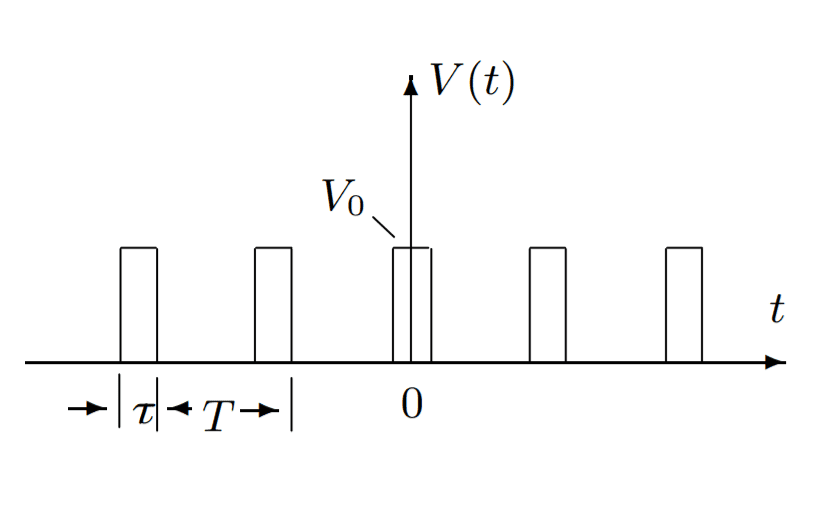
\includegraphics[width=0.9\linewidth]{sp1.png}}
				\caption{Прямоугольные импульсы}
			\end{minipage}
			\begin{minipage}[h]{0.5\linewidth}
				\center{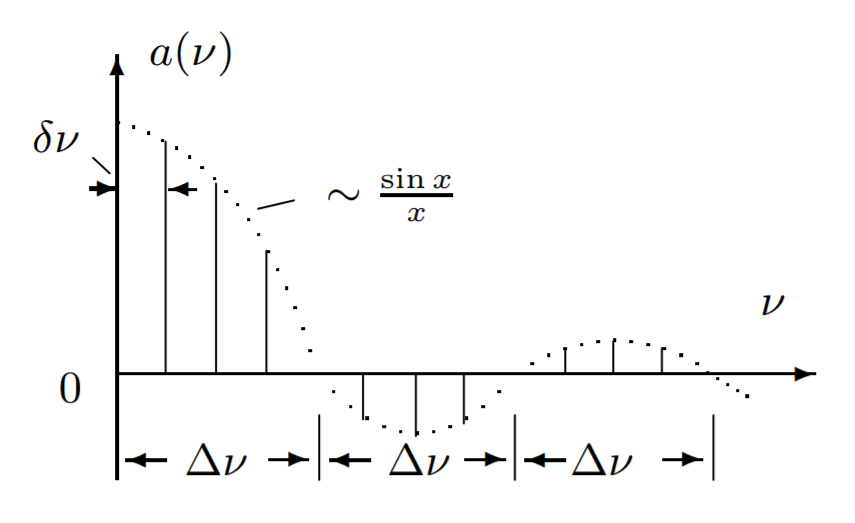
\includegraphics[width=0.9\linewidth]{sp2.png}}
				\caption{Спектр последовательности прямоугольных импульсов}
			\end{minipage}
		\end{figure}
	
	Назовем \textit{шириной спектра} $\Delta \omega$ расстояние от главного максимума ($\omega =0$) до первого нуля огибающей, возникающего при $n=\dfrac{2\pi}{\tau \Omega_{1}}$. При этом 

	$$\Delta \omega \tau \backsimeq 2 \pi $$
	
	 или 
	
\begin{equation}\label{neopr}
	\Delta \nu \Delta t \backsimeq 1
\end{equation}
		
	Полученное соотношение взаимной связи интервалов $\Delta \nu$ и $\Delta t$ является
	частным случаем соотношения неопределенности в квантовой механике.
	
	\item \textbf{Периодическая последовательность цугов} гармонического колебания $V_{0}\cos(\omega_{0}t)$ с длительностью цуга $\tau$ и периодом повторения $T$ (рис. 3).
	
	Функция $f(t)$ снова является четной относительно $t=0$. Коэффициент при $n$-й гармонике равен
\begin{equation}
    a_{n}=\dfrac{2}{T}\int\limits_{-\frac{\tau}{2}}^{\frac{\tau}{2}}V_{0}\cos(\omega_{0}t)\cos(n \Omega_{1} t)dt=V_{0}\dfrac{\tau}{T} \bigg(\dfrac{\sin[(\omega_{0}-n\Omega_{1})\frac{\tau}{2}]}{(\omega_{0}-n\Omega_{1})\frac{\tau}{2}}+\dfrac{\sin[(\omega_{0}+n\Omega_{1})\frac{\tau}{2}]}{(\omega_{0}+n\Omega_{1})\frac{\tau}{2}} \bigg)
\label{eq6}
\end{equation}
	
	Зависимость для случая, когда $\frac{T}{\tau}$ равно целому числу, представлена на рис. 4. Сравнивая спектр последовательности прямоугольных импульсов и цугов мы видим, что они аналогичны, но их максимумы сдвинуты по частоте на величину $\omega_{0}$.
	
	\begin{figure}[h]
		\begin{minipage}[h]{0.5\linewidth}
			\center{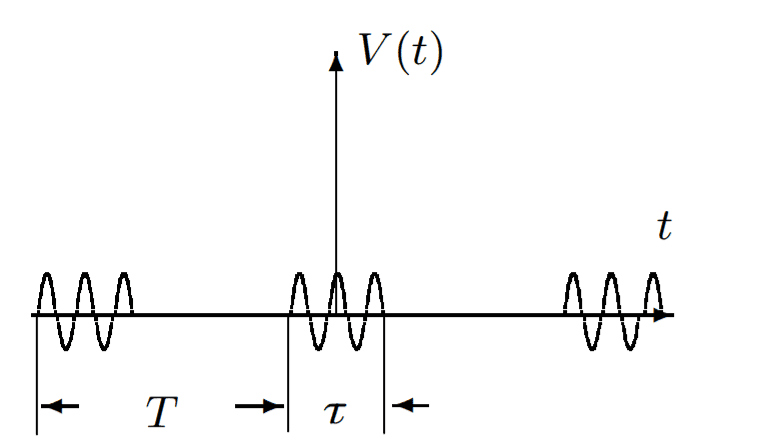
\includegraphics[width=0.9\linewidth]{sp3.png}}
			\caption{Последовательность цугов}
		\end{minipage}
		\begin{minipage}[h]{0.5\linewidth}
			\center{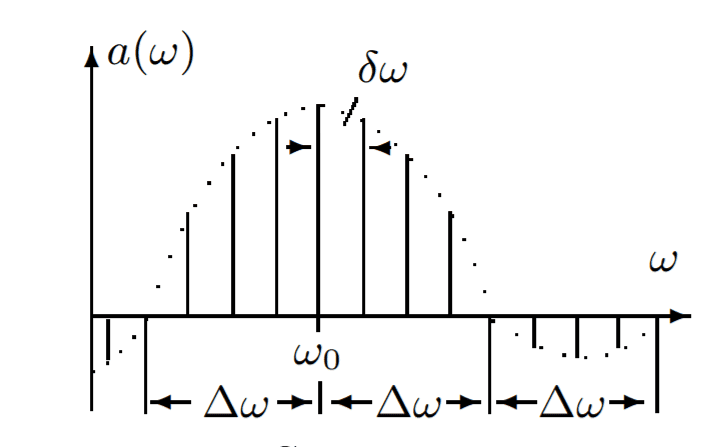
\includegraphics[width=0.9\linewidth]{sp4.png}}
			\caption{Спектр последовательности цугов}
		\end{minipage}
	\end{figure}

	\item \textbf{Амплитудно-модулированные колебания.} Рассмотрим гармонические колебания высокой частоты $\omega_{0}$ , амплитуда которых медленно меняется по гармоническому закону с частотой $\Omega$ ($\Omega \ll \omega_{0})$) (рис. 5):
\begin{equation}
    f(t)=A_{0}[1+m\cos\Omega t]\cos \omega_{0}t
\label{eq7}
\end{equation}	

	Коэффициент $m$ называют \textbf{глубиной модуляции}. При $m<1$ амплитуда колебаний меняется от минимальной $A_{min}=A_{0}(1-m)$ до максимальной $A_{max}=A_{0}(1+m).$ Глубина модуляции может быть представлена в виде
	
\begin{equation}\label{m}
	 m=\dfrac{A_{max}-A_{min}}{A_{max}+A_{min}}
\end{equation}
	
	Простым тригонометрическим преобразованием можно найти спектр амплитудно - модулированных колебаний:
	\\
\begin{equation}\label{a}
	f(t)=A_{0}\cos(\omega_{0} t)+\dfrac{A_{0}m}{2}\cos(\omega_{0}+\Omega)t+\dfrac{A_{0}m}{2}\cos(\omega_{0}-\Omega)t.
\end{equation}
		
		\begin{figure}[h]
			\begin{minipage}[h]{0.5\linewidth}
				\center{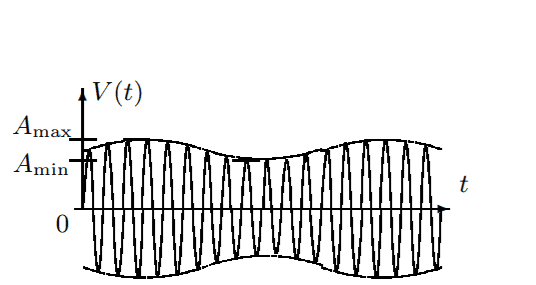
\includegraphics[width=0.9\linewidth]{sp5.png}}
				\caption{Модулированные гармонические колебания}
			\end{minipage}
			\begin{minipage}[h]{0.5\linewidth}
				\center{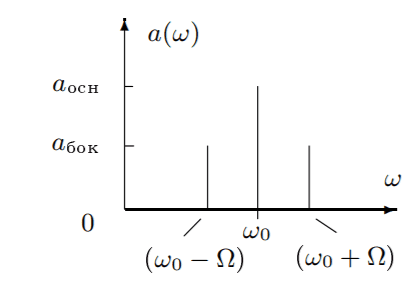
\includegraphics[width=0.9\linewidth]{sp6.png}}
				\caption{Спектр модулированных гармонических колебаний}
			\end{minipage}
		\end{figure}
		
		Спектр таких колебаний содержит три составляющих  основную
		компоненту и две боковых (рис. 6). Первое слагаемое в правой части представляет собой исходное немодулированное колебание
		с основной (несущей) частотой $\omega_{0}$ и амплитудой $a_{осн} = A_{0}$ . Второе и третье слагаемые соответствуют новым гармоническим колебаниям с частотами $\omega_{0} + \Omega$ и $\omega_{0} - \Omega$. Амплитуды этих двух колебаний одинаковы и составляют $\dfrac{m}{2}$ от амплитуды немодулированного колебания:
		$a_{бок} = \dfrac{A_{0}m}{2}$. Начальные фазы всех трех колебаний одинаковы.
	\end{enumerate}

\section{Ход работы}

\subsection*{А. Исследование спектра периодической последовательности
прямоугольных импульсов и проверка соотношений неопределённости}

\begin{enumerate}

\item [\textbf{1.}]  Настраиваем генератор на прямоугольные импульсы с частотой повторения $\nu_\text{повт}$ = 1 кГц (период $T$ = 1 мс) и
длительностью импульса $\tau$ = $T$/20 = 50 мкс.

\item [\textbf{2.}] Получаем на экране спектр (Преобразование Фурье) сигнала.

\textbf{a.} Изменяем $\nu_\text{повт}$ при фиксированном $\tau$ = 50 мкс и получаем:

\begin{figure}[h]
\begin{minipage}[h]{0.47\linewidth}
\center{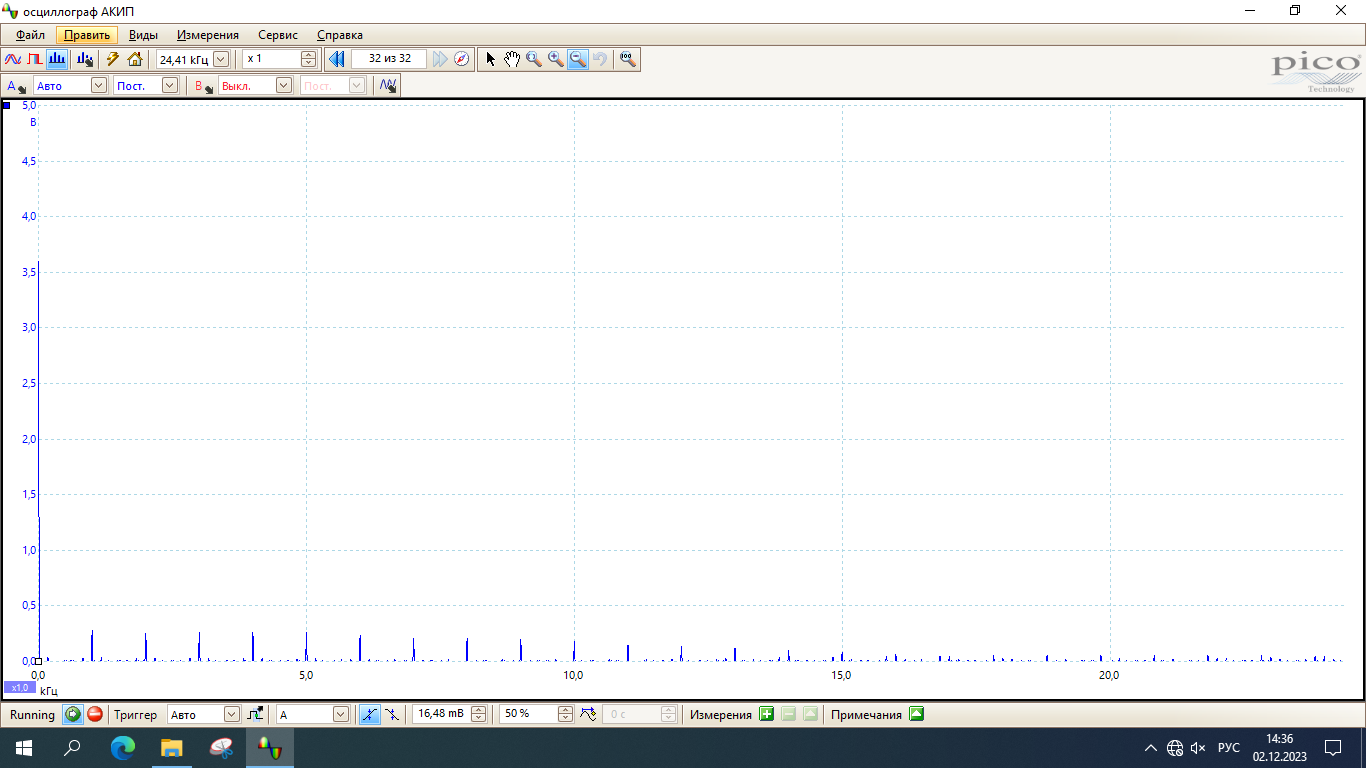
\includegraphics[width=1\linewidth]{A_1k_50.png}}  \\$\nu_\text{повт}$ = 1 кГц 
\end{minipage}
\hfill
\begin{minipage}[h]{0.47\linewidth}
\center{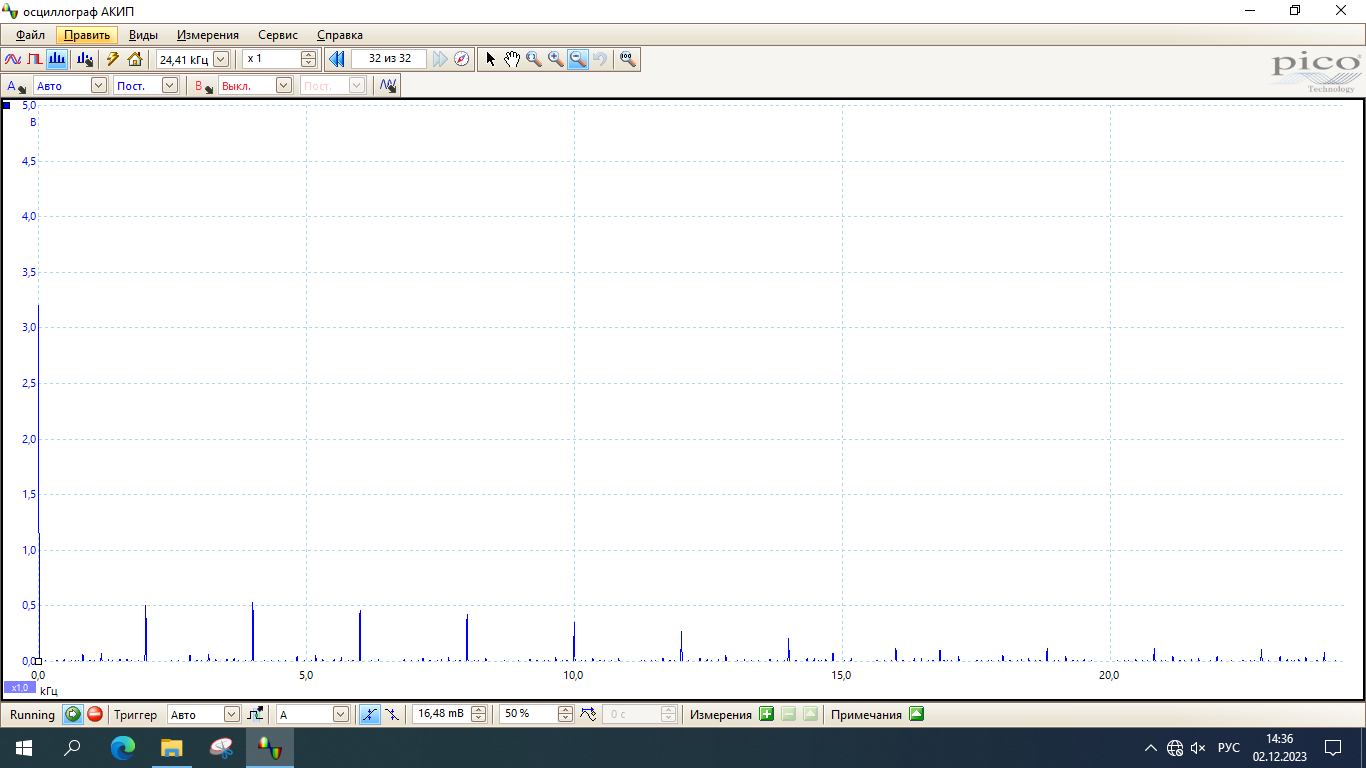
\includegraphics[width=1\linewidth]{A_2k_50.png}} \\$\nu_\text{повт}$ = 2 кГц 
\end{minipage}
\vfill
\begin{minipage}[h]{0.47\linewidth}
\center{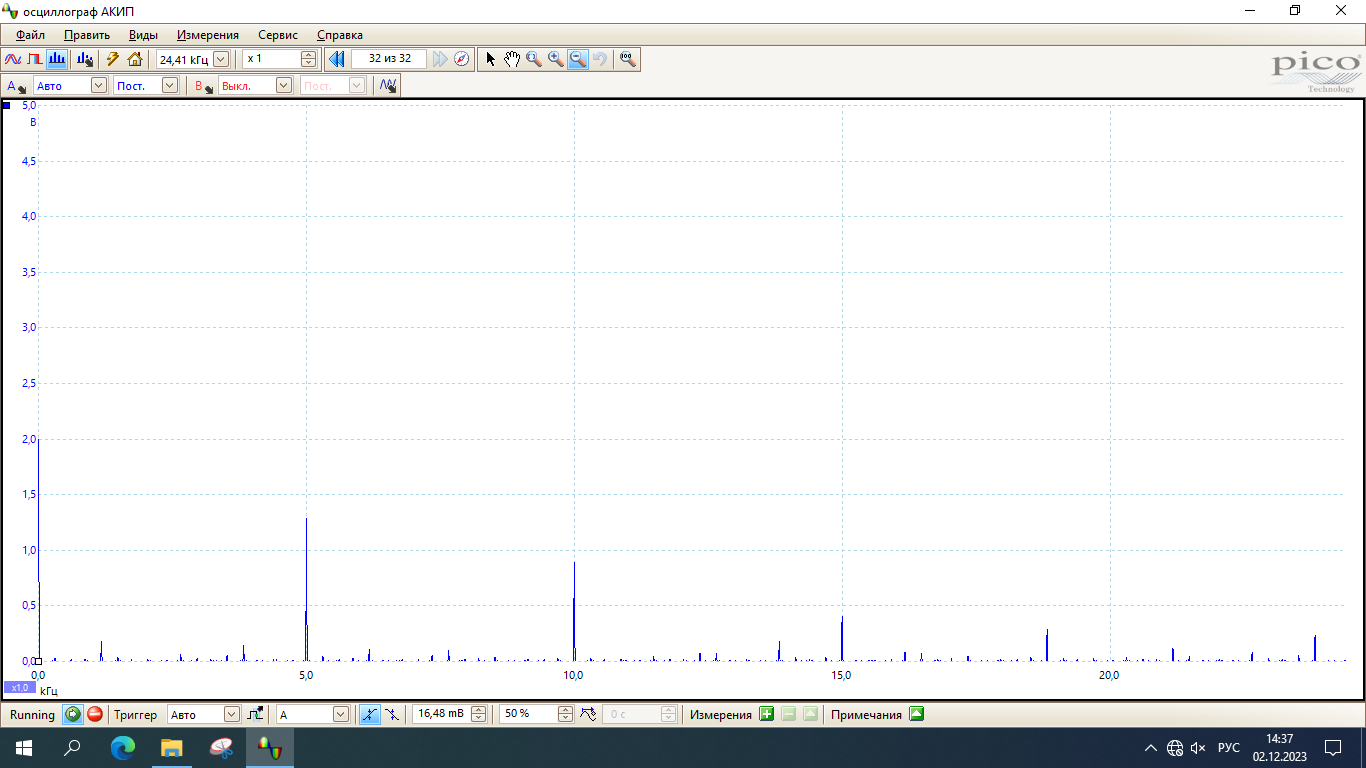
\includegraphics[width=1\linewidth]{A_5k_50.png}} $\nu_\text{повт}$ = 5 кГц  \\
\end{minipage}
\hfill
\begin{minipage}[h]{0.47\linewidth}
\center{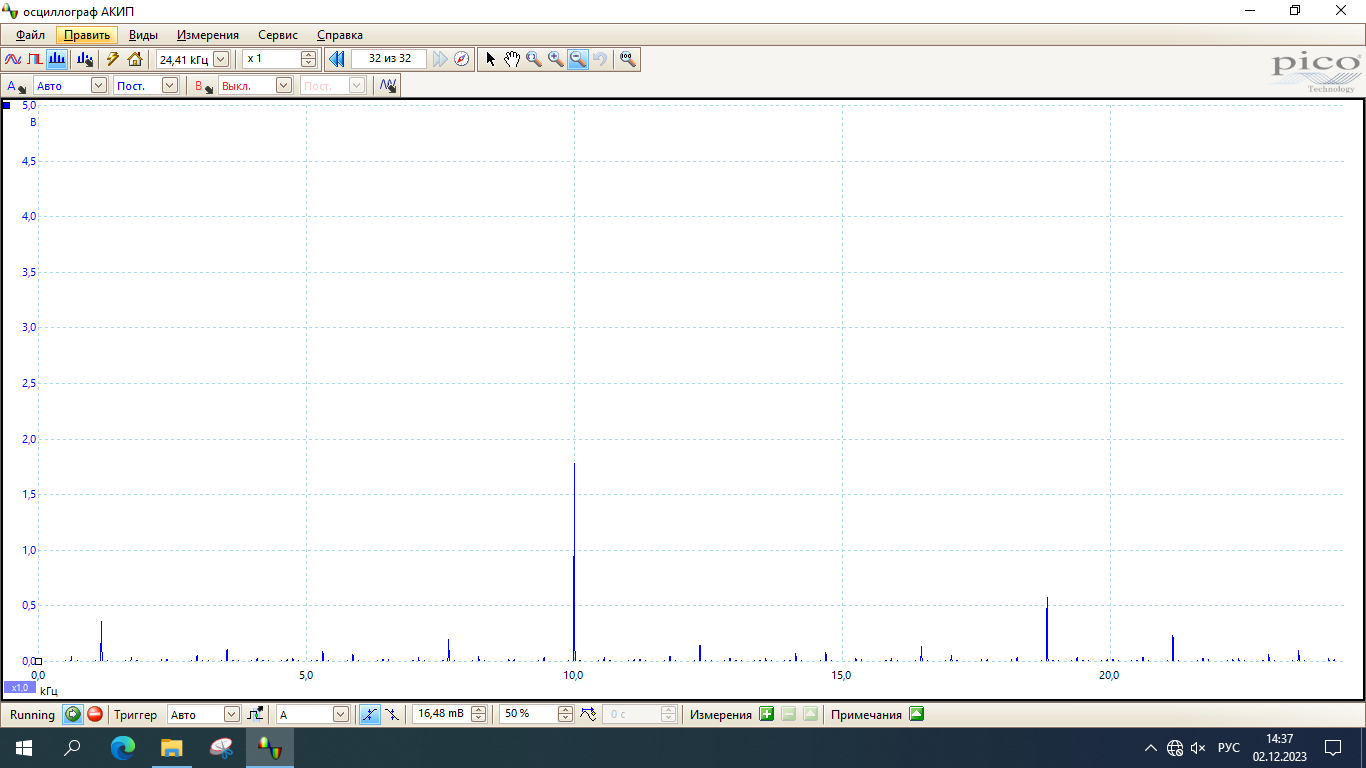
\includegraphics[width=1\linewidth]{A_10k_50.png}} $\nu_\text{повт}$ = 10 кГц  \\
\end{minipage}
\caption{}
\label{ris:experimentalcorrelationsignals}
\end{figure}


Как видно из графиков, при увеличении частоты повторения сигнала увеличивается расстояние между компонентами спектра.

\newpage


\textbf{б.} Изменяем $\tau$ при фиксированном $\nu_\text{повт}$ = 1 кГц и получаем:

\begin{figure}[h]
\begin{minipage}[h]{0.47\linewidth}
\center{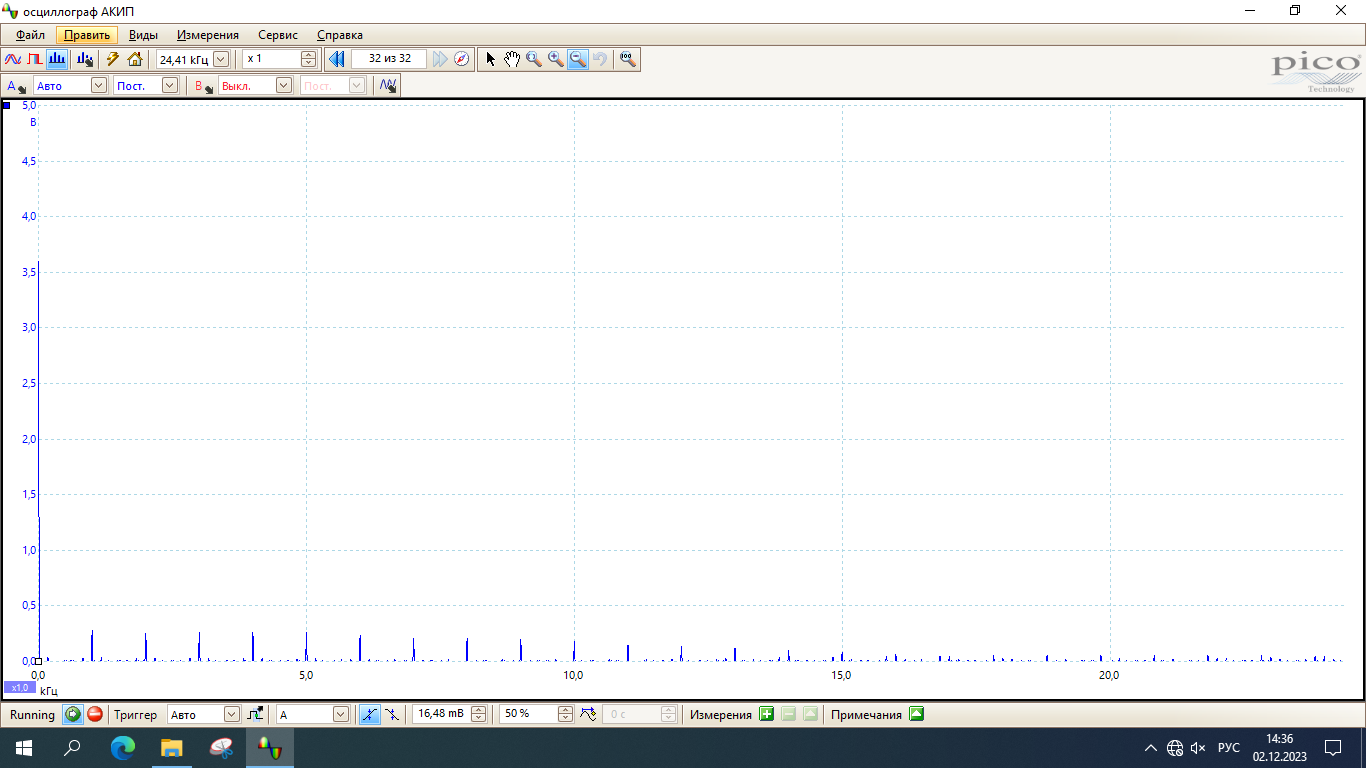
\includegraphics[width=1\linewidth]{A_1k_50.png}} $\tau$ = 50 мкс \\
\end{minipage}
\hfill
\begin{minipage}[h]{0.47\linewidth}
\center{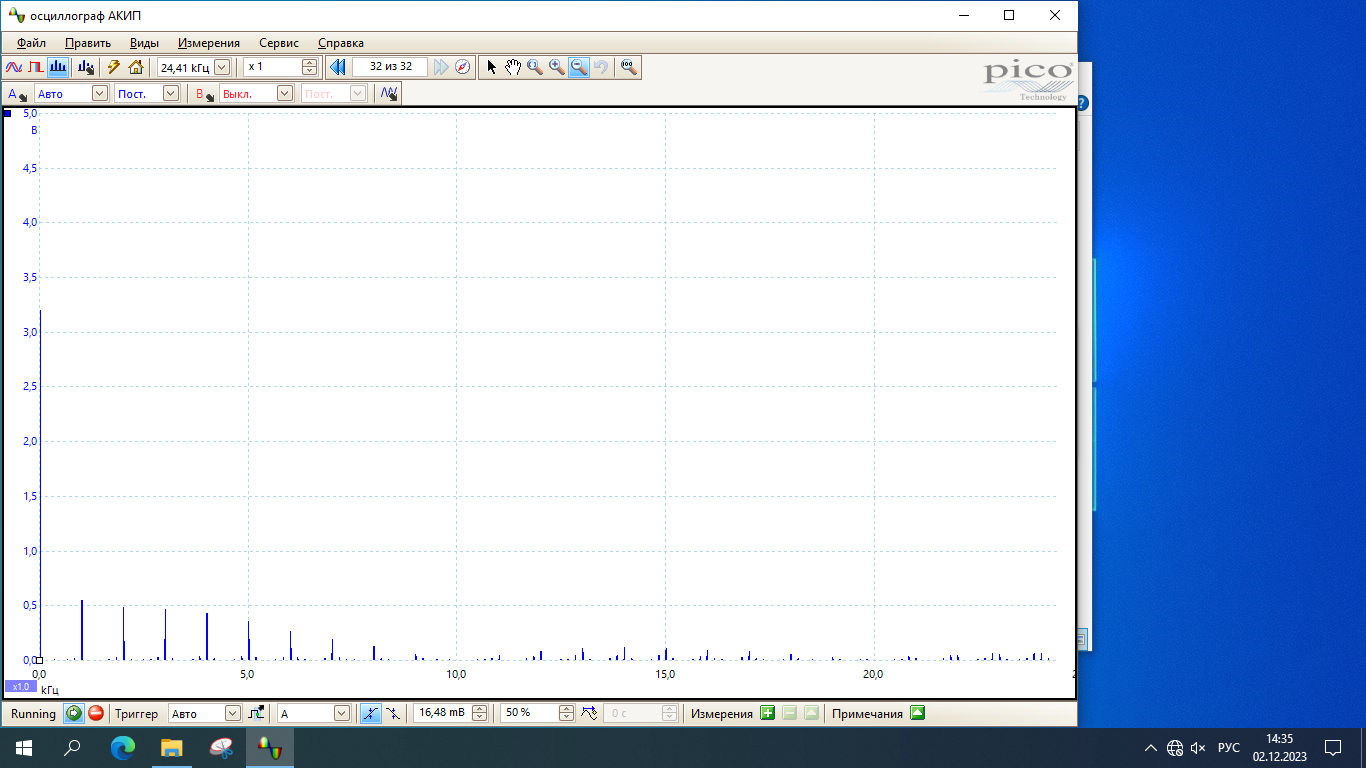
\includegraphics[width=1\linewidth]{A_1k_100.png}} \\ $\tau$ = 100 мкс
\end{minipage}
\vfill
\begin{minipage}[h]{0.47\linewidth}
\center{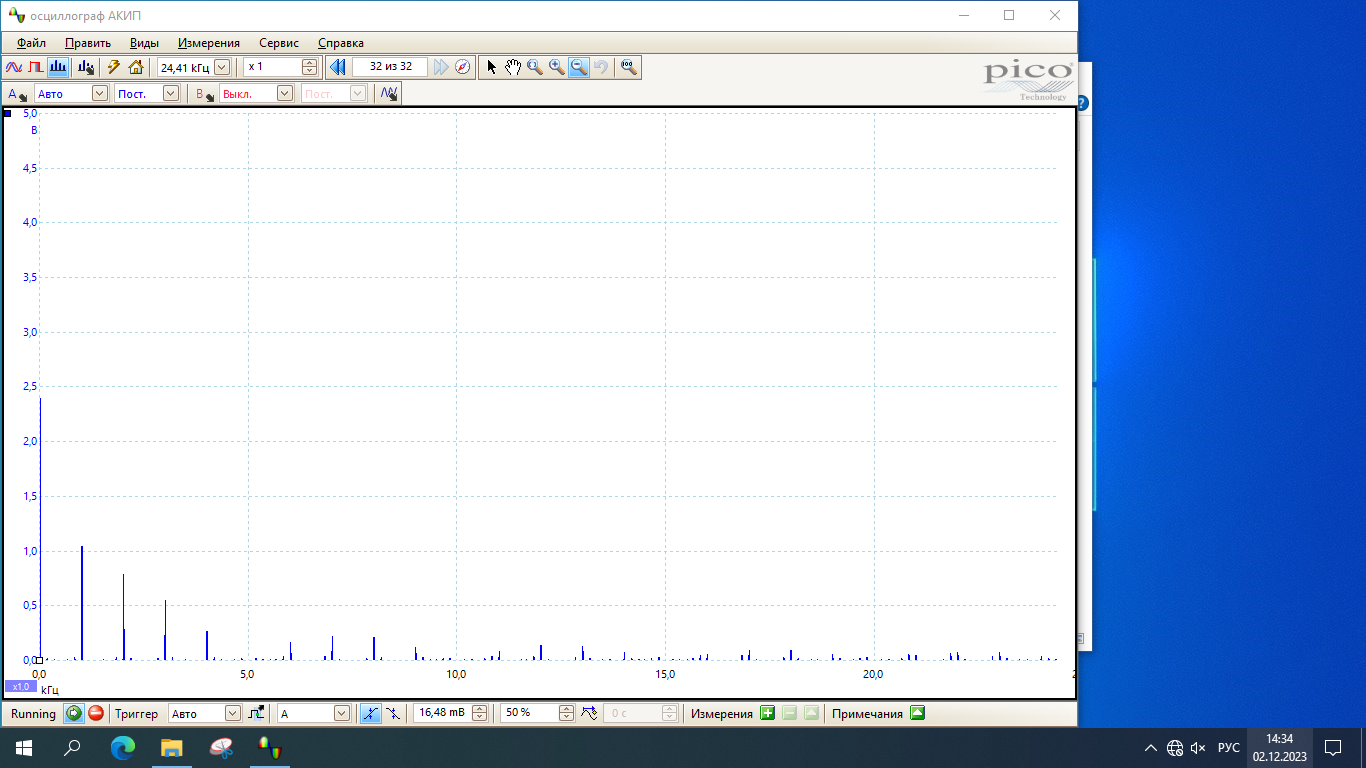
\includegraphics[width=1\linewidth]{A_1k_200.png}} $\tau$ = 200 мкс \\ 
\end{minipage}
\caption{}
\label{ris:experimentalcorrelationsignals}
\end{figure}

Как видно из графиков, при увеличении длительности сигнала уменьшается ширина спектра.

\item [\textbf{3.}] Измерим амплитуды $a_n$ и частоты $\nu_n$ спектральных гармоник при фиксированных $\nu_\text{повт}$ = 3кГц и $\tau$ = 50 мкс.

\begin{table}[!h]
\centering
\begin{tabular}{|l|l|l|l|l|l|l|}
\hline
$n$ гармоники & 1 & 2 & 3 & 4 & 5 & 6\\ \hline
$\nu_n^\text{эксп}$, кГц & 3.0 & 6.0 & 9.0 & 12.0 & 15.0 & 18.8 \\ \hline
$\nu_n^\text{теор}$, кГц & 3. & 6.0 & 9.0 & 12.0 & 15.0 & 18.0 \\ \hline
$|a_n|^\text{эксп}$, мВ & 791 & 699 & 607 & 414 & 240 & 174\\ \hline
$|a_n/a_1|_\text{эксп}$ & 1 & 0.884 & 0.767 & 0.523 & 0.303 & 0.220 \\ \hline
$|a_n/a_1|_\text{теор}$ & 1 & 0.891 & 0.725 & 0.524 & 0.312 & 0.114\\ \hline
\end{tabular}
\end{table}

Здесь $a_1$ = 143.8 мВ.
$$\nu_n^\text{теор} = \frac{n}{T}$$
$$|a_n|_\text{теор} = \frac{|\text{sin}\frac{\pi n \tau}{T}|}{\pi n}$$

\item[\textbf{4.}] Зафиксируем период повторения прямоугольного сигнала $T = 1 \text{мс}$, $\nu_\text{повт} = 1\text{кГц}$. Изменяя длительность импульса $\tau$ в диапазоне от 
$\tau=T/50$ до $\tau=T/5$, измерим полную ширину спектра сигнала $\Delta \nu$ — от центра спектра ($\nu = 0$) до гармоники с нулевой амплитудой $a_n \approx 0$ и установим зависимость между $\Delta \nu$ и $\tau$, полученную из формулы \ref{eq5}.

\begin{table}[h!]
    \centering
    \begin{tabular}{|c|c|c|c|c|c|c|c|}
\hline
$\tau$, мкс & 20 & 40 & 60 & 80 & 100 & 120 & 140 \\ \hline
$\Delta \nu$, кГц & 50 & 25 & 17 & 12.5 & 10 & 7.5 & 5 \\ \hline
$1/\tau \cdot 10^3$, с$^{-1}$ & 50.0 & 25.0 & 16.7 & 12.5 & 10 & 8.3 & 7.1 \\ \hline
\end{tabular}
    \caption{Исследование зависимости $\Delta \nu$ и $\tau$}
    \label{table2}
\end{table}
Построим график $\Delta\nu\left(\frac{1}{\tau}\right)$. Используя МНК, получим $k=1.0229\pm0,0223$, откуда с хорошей точностью можем заключить, что $\Delta\nu\frac{1}{\tau}=1$, что экспериментально доказывает соотношение неопределённостей. График приведён на рис.12
\begin{figure}[h]
    \centering
    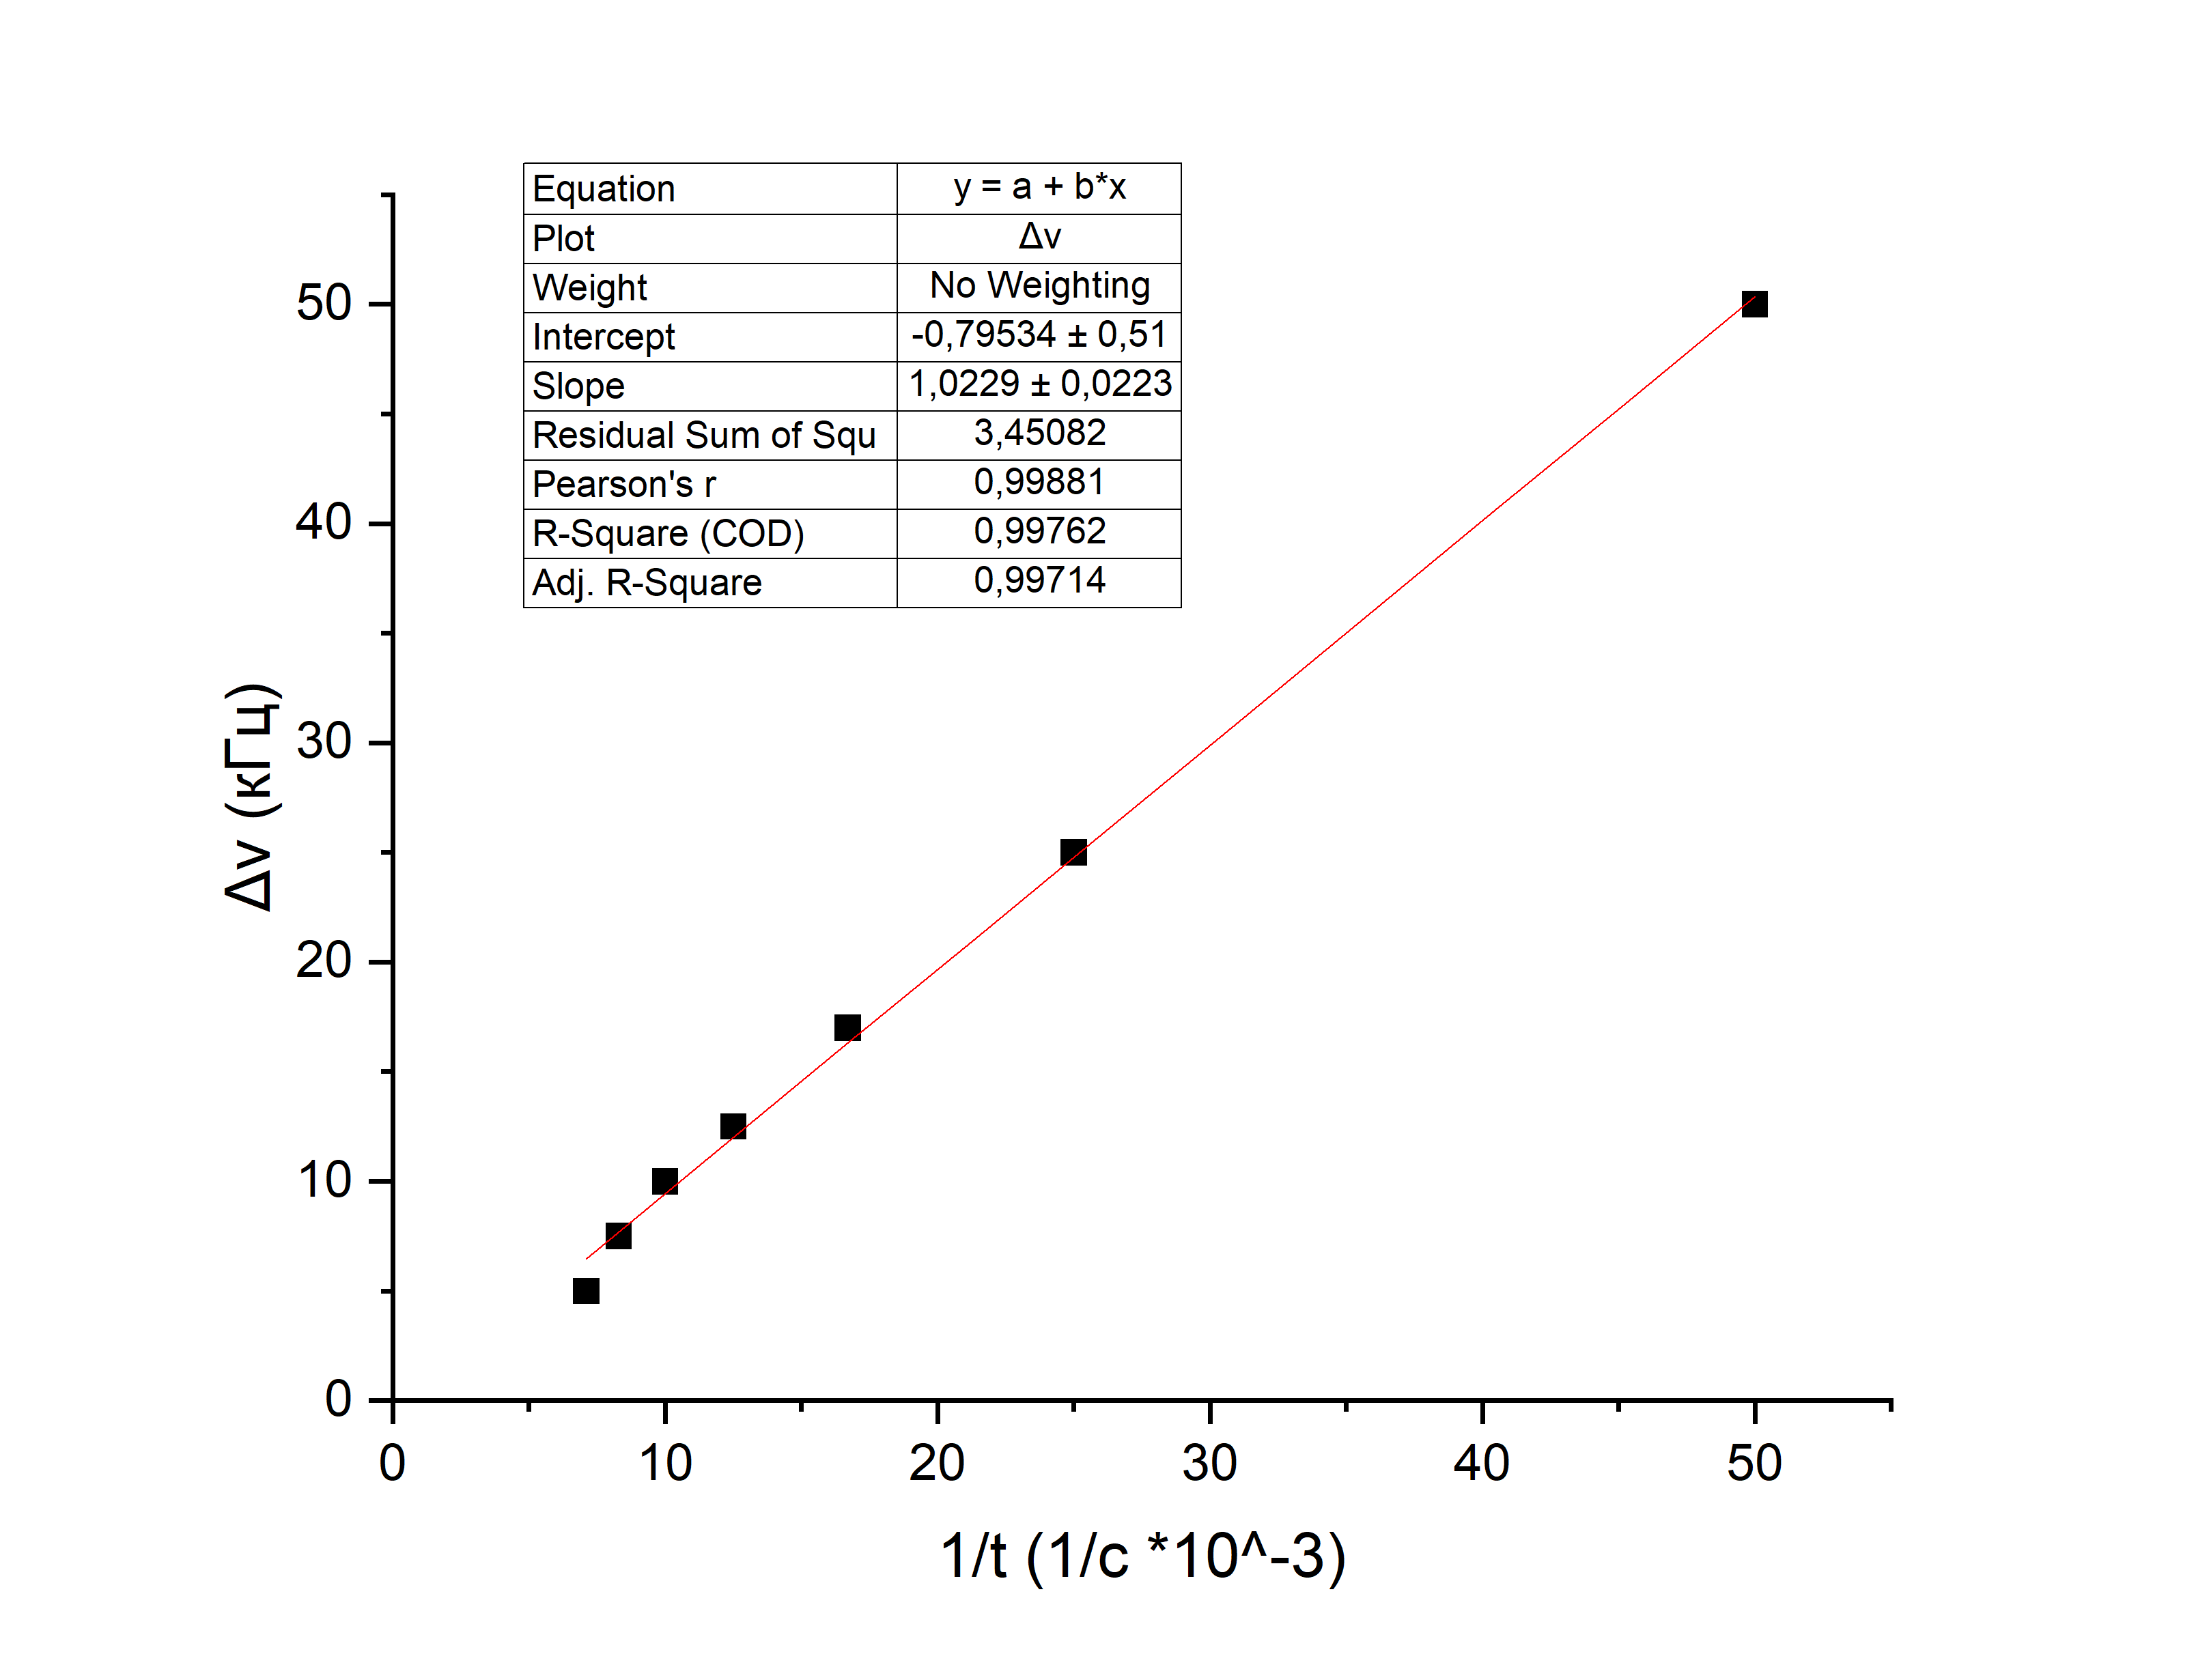
\includegraphics[width=0.7\linewidth]{grafic1.png}
    \caption{Зависимость $\Delta \nu$ от $1/\tau$}
    \label{grafic1}
\end{figure}

\item[\textbf{5.}] 
Зафиксируем длительность импульса прямоугольного сигнала $\tau = 100 \text{мкс}$. Изменяя период повторения $T$ в диапазоне от $2\tau$ до $50\tau$ измерим расстояния $\delta\nu = \nu_{n+1} - \nu_n$ между соседними гармониками спектра. 
\begin{table}[h!]
    \centering
    \begin{tabular}{|c|c|c|c|c|c|c|c|c|c|c|c|}
\hline
$T$, мкс & 200 & 500 & 1000 & 1500 & 2000 & 2500 & 3000 & 3500 & 4000 & 4500 & 5000 \\ \hline
$\delta \nu$, кГц & 5 & 2 & 1 & 0.688 & 0.459 & 0.400 & 0.330 & 0.287& 0.250 & 0.220& 0.200 \\ \hline
\end{tabular}
    \caption{Зависимость $\delta \nu$ от $T$}
    \label{table3}
\end{table}

\newpage

\begin{figure}[h]
    \centering
    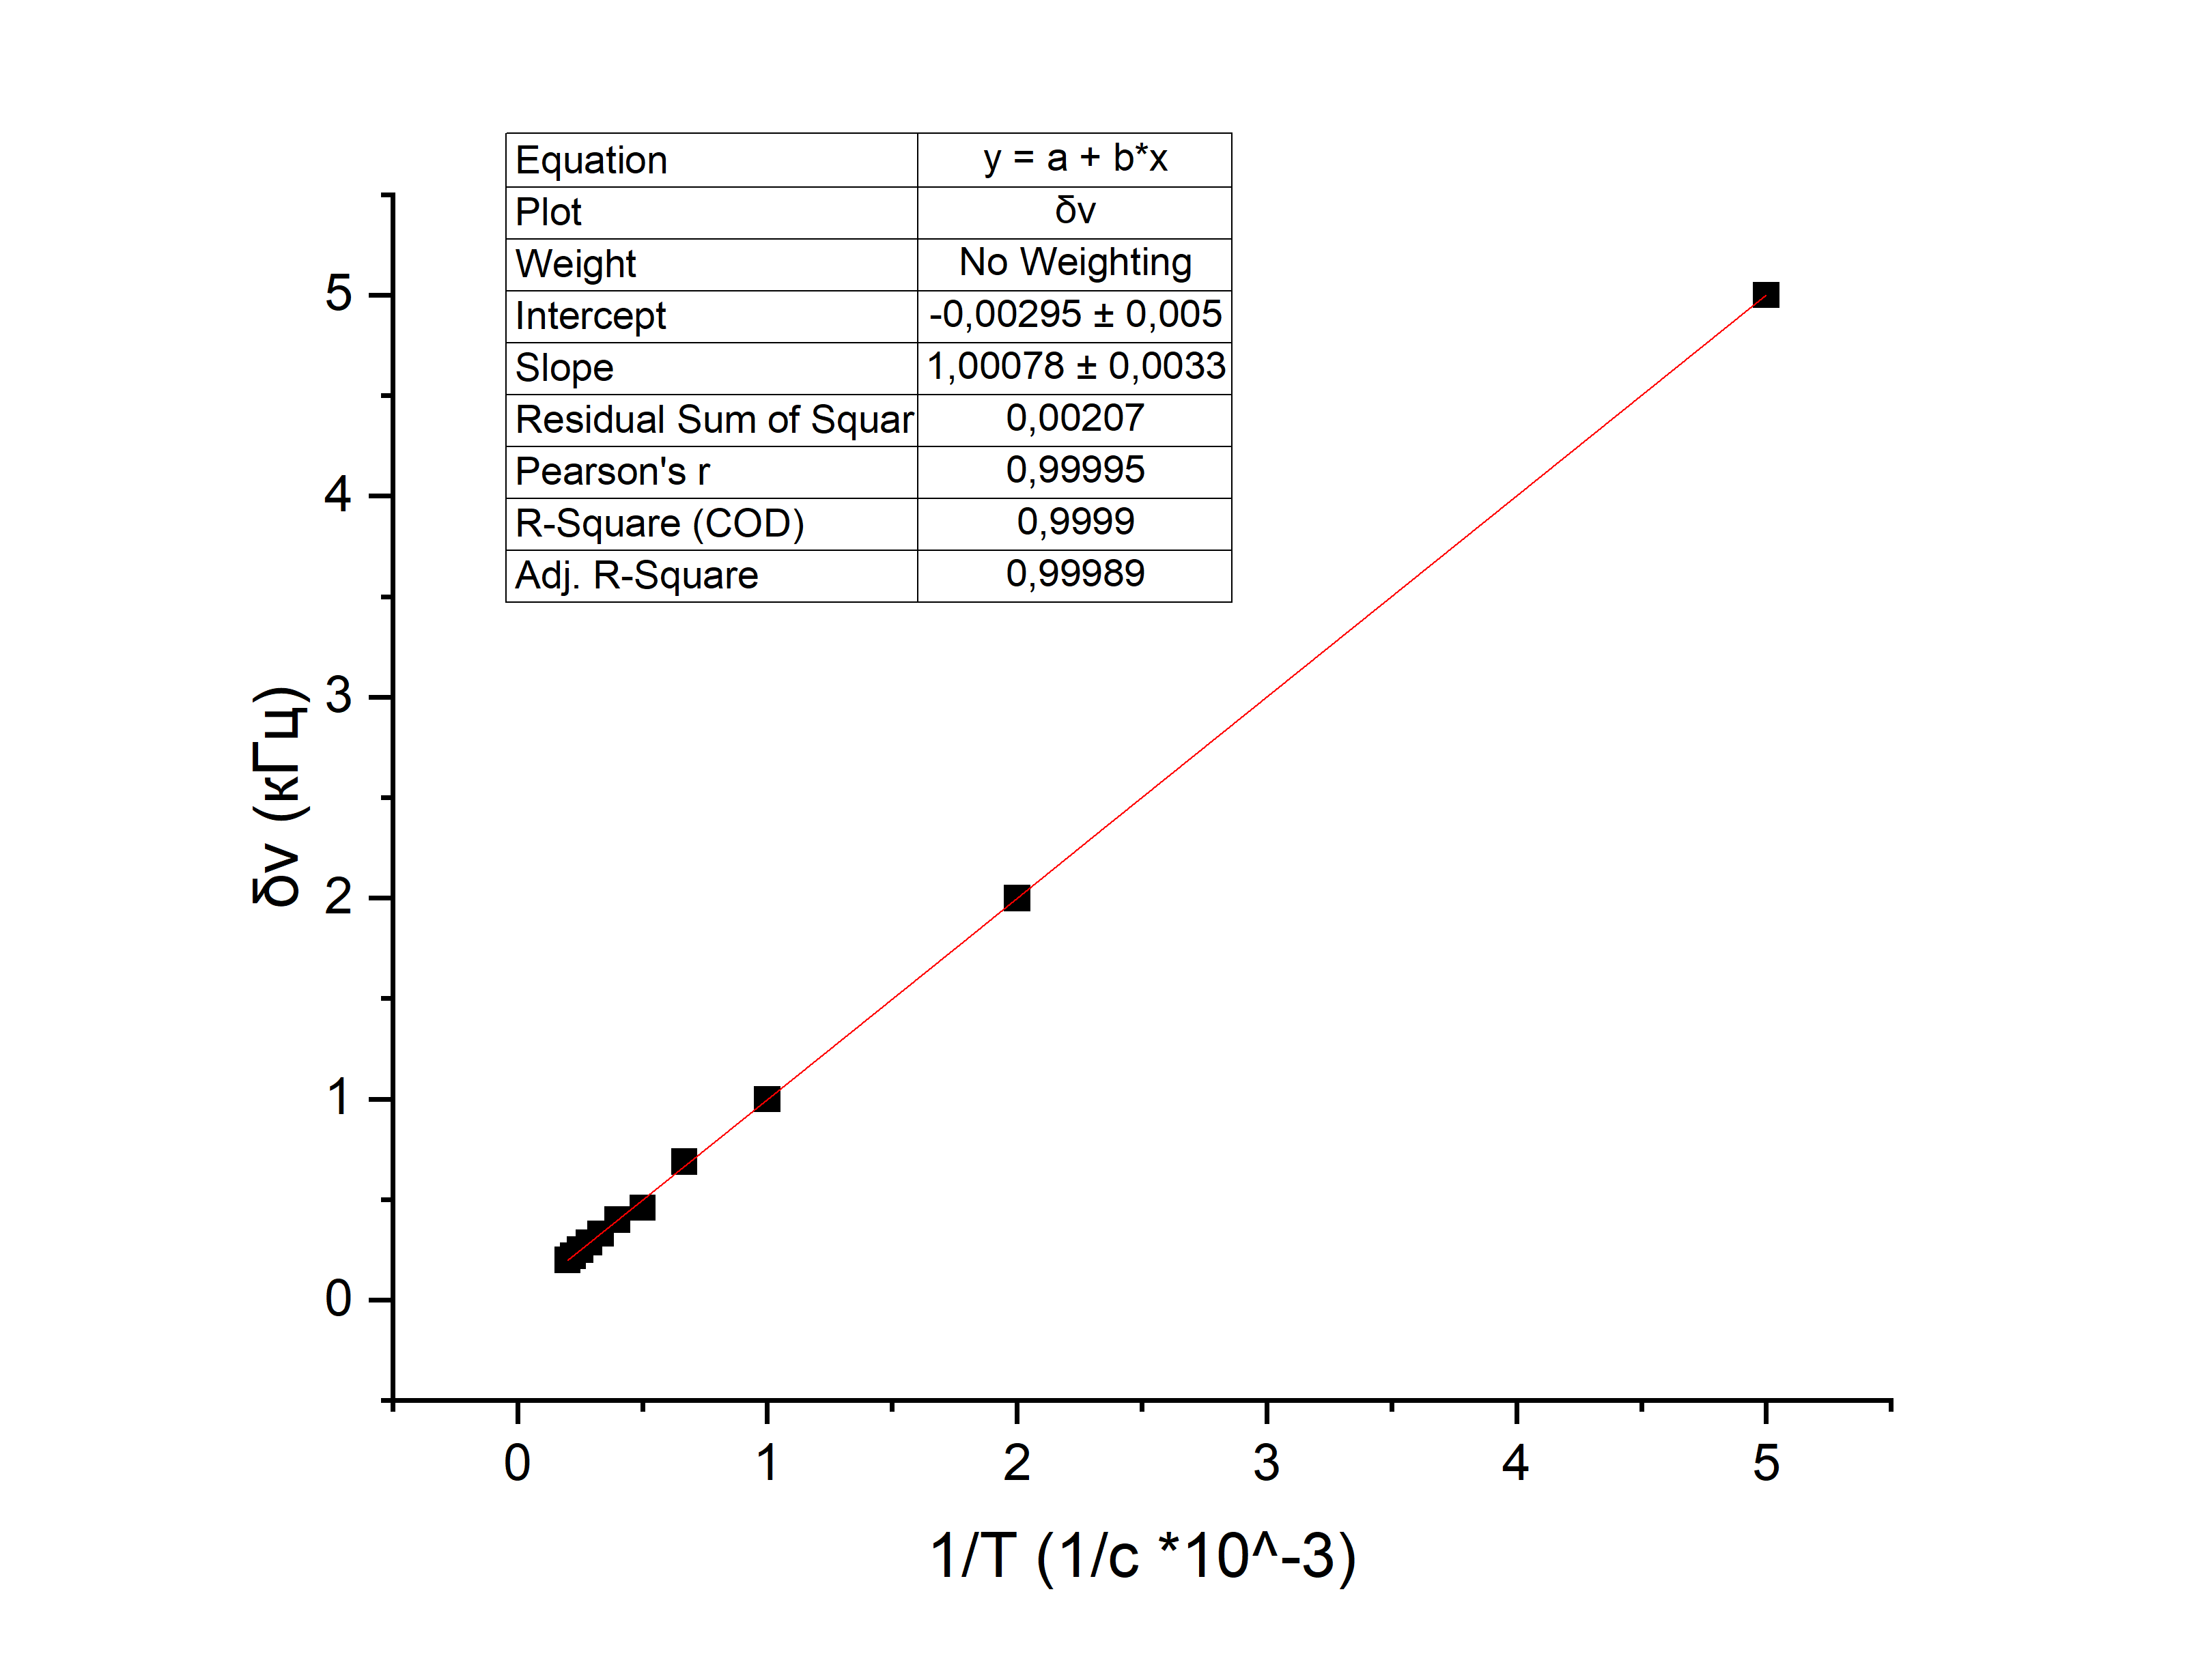
\includegraphics[width=0.7\linewidth]{grafic2.png}
    \caption{Зависимость $\delta \nu$ от $1/T$}
    \label{grafic2}
\end{figure}
Построим график $\delta\nu\left(\frac{1}{T}\right)$. Используя МНК, получим $k=1.001\pm0.003$, что экспериментально доказывает соотношение неопределённостей. График приведён на рис.13.
\end{enumerate}


\newpage

\subsection*{Г. Наблюдение спектра амплитудно-модулированного сигнала}


\begin{enumerate}


\item [\textbf{1.}] Настраиваем генератор в режим модулированного по амплитуде синусоидального сигнала с несущей частотой $\nu_0$ = 50 кГц, частотой модуляции $\nu_\text{мод}$ = 2 кГц и глубиной модуляции $m$ = 0.5.

\item [\textbf{2.}] Получаем на экране спектр (Преобразование Фурье) сигнала. Из графика получим $A_{max} = 1.489 \text{мВ}$ и $A_{min} = 0.489 \text{мВ}$ и убедимся в справедливости соотношения $$ m = \frac{A_\text{max} - A_\text{min}}{A_\text{max} + A_\text{min}} = \frac{1}{1.978} \approx 0.5 $$
Поскольку мы установили глубину модуляции на $0,5$, а из теории у нас получилась $0,503$, то мы видим, что формула \ref{eq8} верна.

\item [\textbf{3.}]
Изменяя на генераторе глубину модуляции $m$ в диапазоне от 10 \% до 100 \% (всего 6-8 точек), измерим отношение амплитуд боковой и основной 
спектральных линий $a_{\text{бок}}/a_{\text{осн}}$. Построим график зависимости $a_{\text{бок}}/a_{\text{осн}}$ от $m$ и проверим, совпадает ли 
результат с теоретическим.

\begin{center}
\begin{tabular}{|c|c|c|c|c|c|c|c|}
\hline
$m$, \% & 10 & 25 & 40 & 55 & 70 & 85 & 100 \\ \hline
$a_{\text{бок}}$, мВ & 33.72 & 84.0 & 135.0 & 186.0 & 235.0 & 285.0 & 334.0 \\ \hline
\multicolumn{8}{|c|}{$a_{\text{осн}}$ = 672 мВ} \\ \hline
$a_{\text{бок}}/a_{\text{осн}}$ & 0.050 & 0.125 & 0.200 & 0.277 & 0.350 & 0.425 & 0.498 \\ \hline
\end{tabular}

\textbf{Таблица 3.} Исследование зависимости $a_{\text{бок}}/a_{\text{осн}}$ от $m$.
\end{center}
\begin{figure}[h]
    \centering
    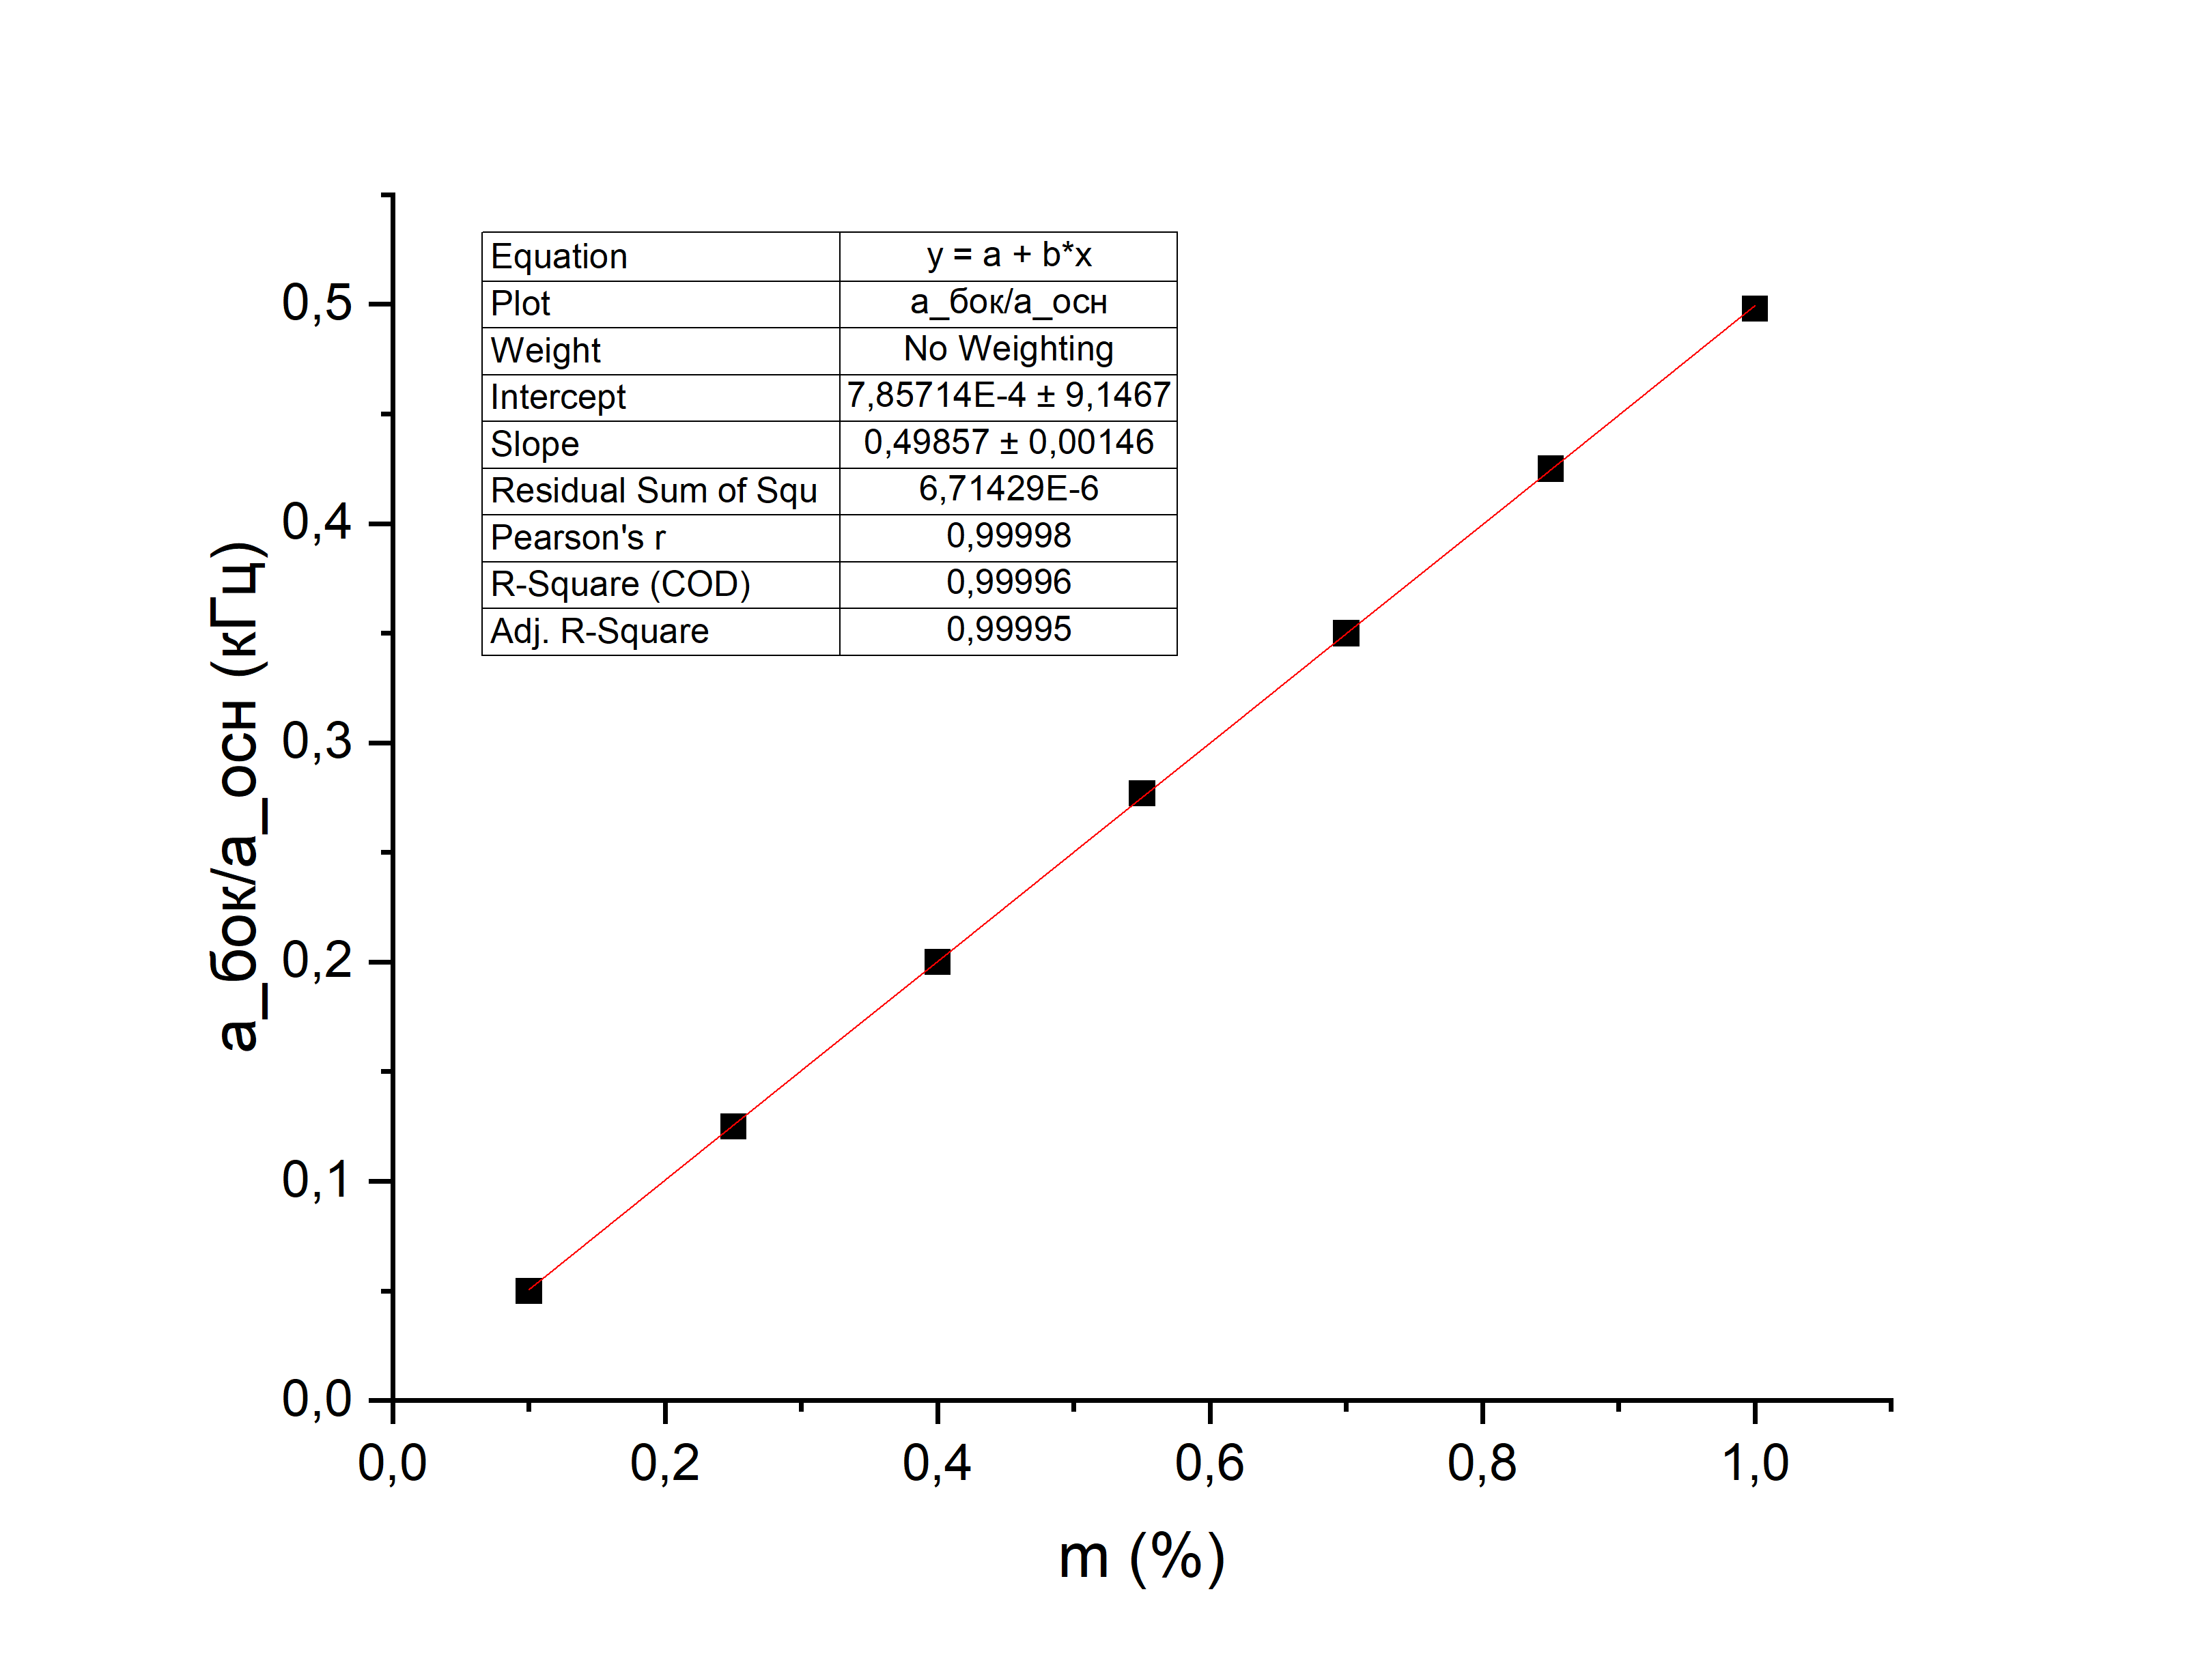
\includegraphics[width=0.7\linewidth]{grafic3.png}
    \caption{Зависимость $a_{\text{бок}}/a_{\text{осн}}$ от $m$}
    \label{grafic3}
\end{figure}
Построим график $\frac{a_{\text{бок}}}{a_{\text{осн}}}(m)$. Используя МНК, получим $k=0.499x\pm0,001$, что подтверждает $\frac{a_{\text{бок}}}{a_{\text{осн}}}=\frac{m}{2}$, т.е. совпадает с теоретическим предсказанием. График приведён на рис.\ref{grafic3}.




\end{enumerate}








\newpage



\subsection*{Д. Наблюдение спектра сигнала, модулированного по фазе}



\begin{enumerate}


\item [\textbf{1.}] Настраиваем генератор в режим модулированного по фазе синусоидального сигнала с несущей частотой $\nu_0$ = 50 кГц, частотой модуляции $\nu_\text{мод}$ = 2 кГц и максимальным отклонением (глубиной модуляцией) $\varphi$ = 10$\degree$.

\item [\textbf{2.}] Получаем на экране спектр (Преобразование Фурье) сигнала.

\begin{figure}[h]
\begin{minipage}[h]{0.44\linewidth}
\center{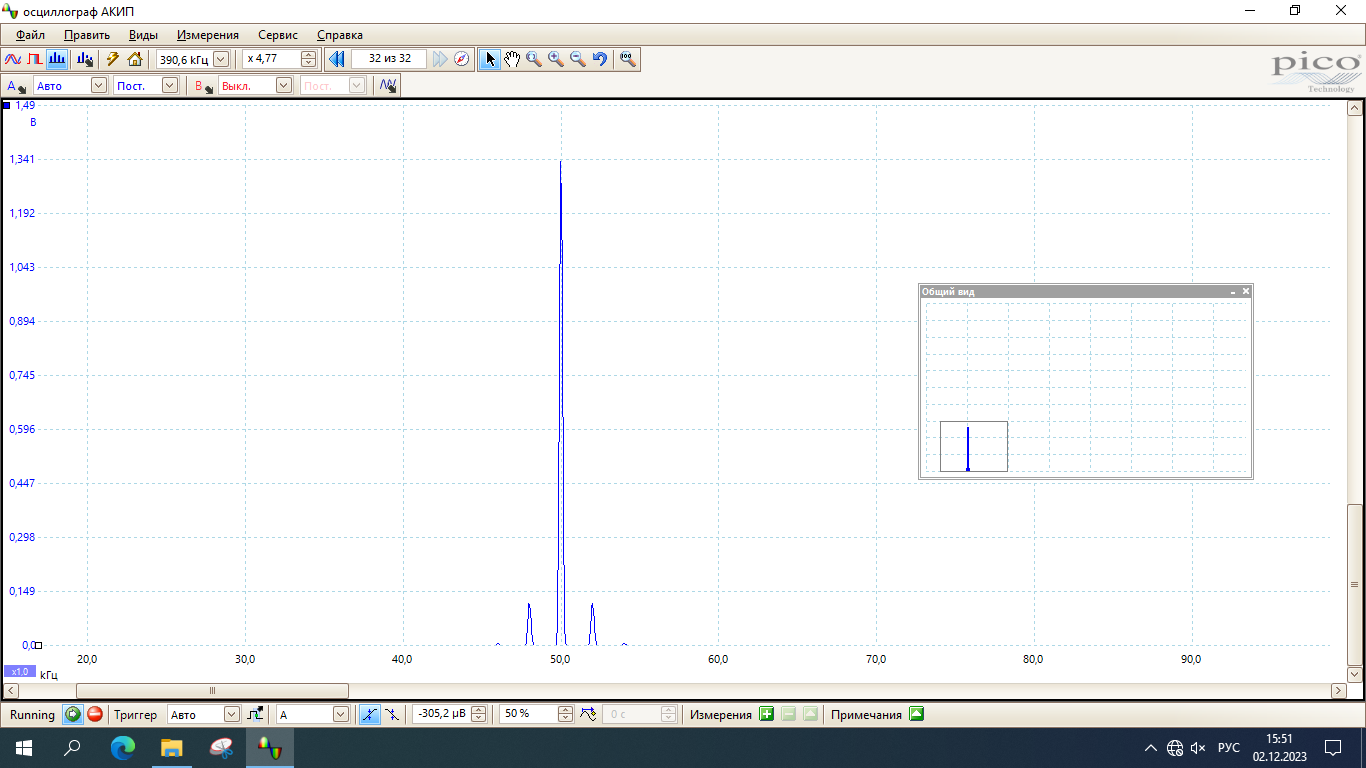
\includegraphics[width=1\linewidth]{D_50k_2k_10f.png}} $\nu_0$ = 50 кГц, $\nu_\text{мод}$ = 2 кГц, $\varphi$ = 10$\degree$  \\
\end{minipage}
\hfill
\begin{minipage}[h]{0.44\linewidth}
\center{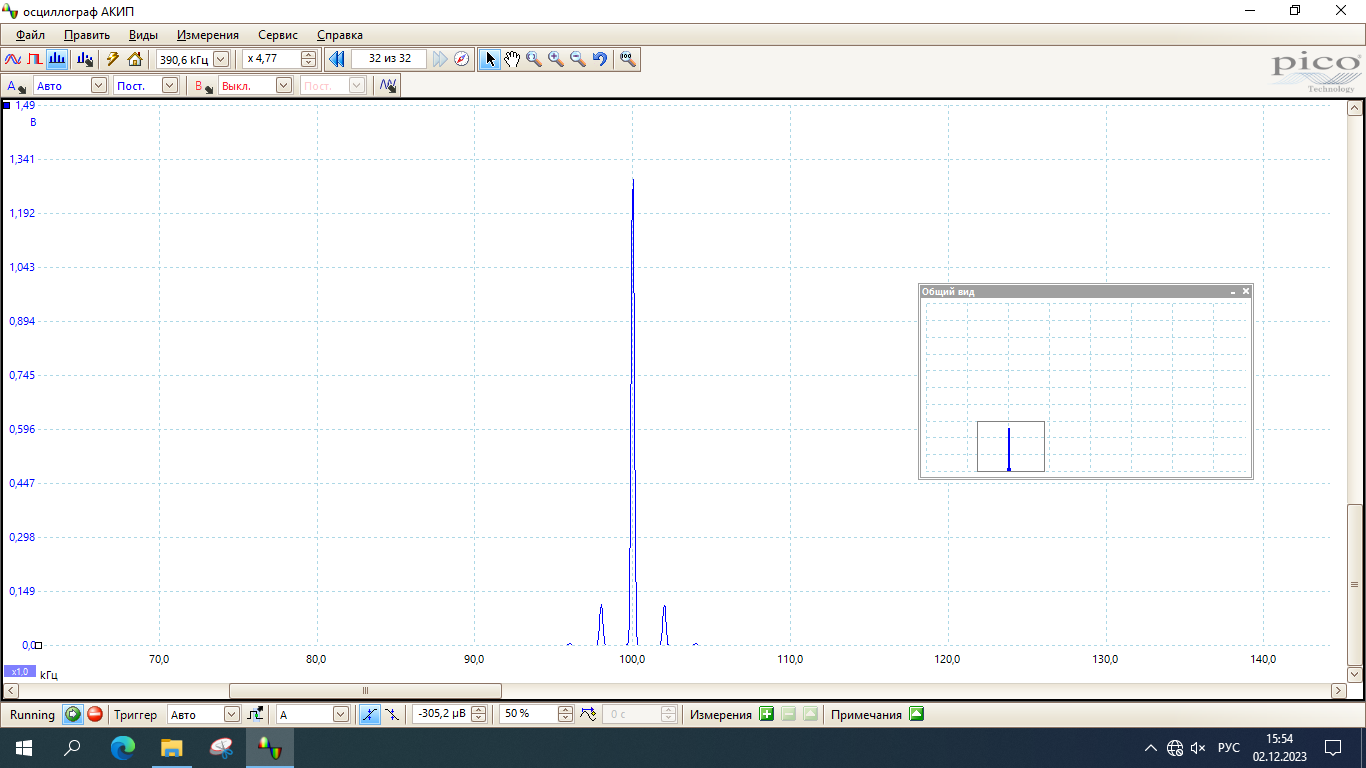
\includegraphics[width=1\linewidth]{D_100k_2k_10f.png}} \\  $\nu_0$ = 100 кГц, $\nu_\text{мод}$ = 2 кГц, $\varphi$ = 10$\degree$   
\end{minipage}
\vfill
\begin{minipage}[h]{0.44\linewidth}
\center{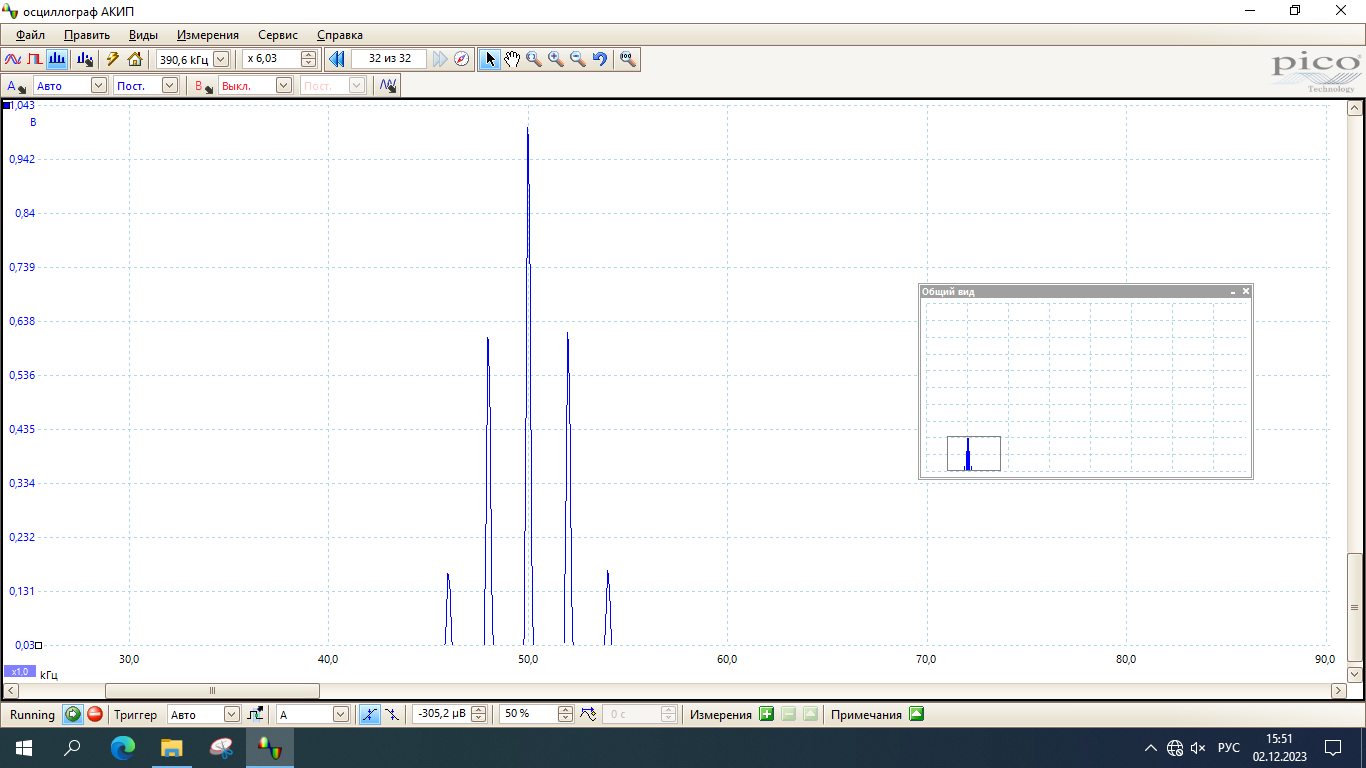
\includegraphics[width=1\linewidth]{D_50k_2k_60f.png}} $\nu_0$ = 50 кГц, $\nu_\text{мод}$ = 2 кГц, $\varphi$ = 60$\degree$   \\
\end{minipage}
\hfill
\begin{minipage}[h]{0.44\linewidth}
\center{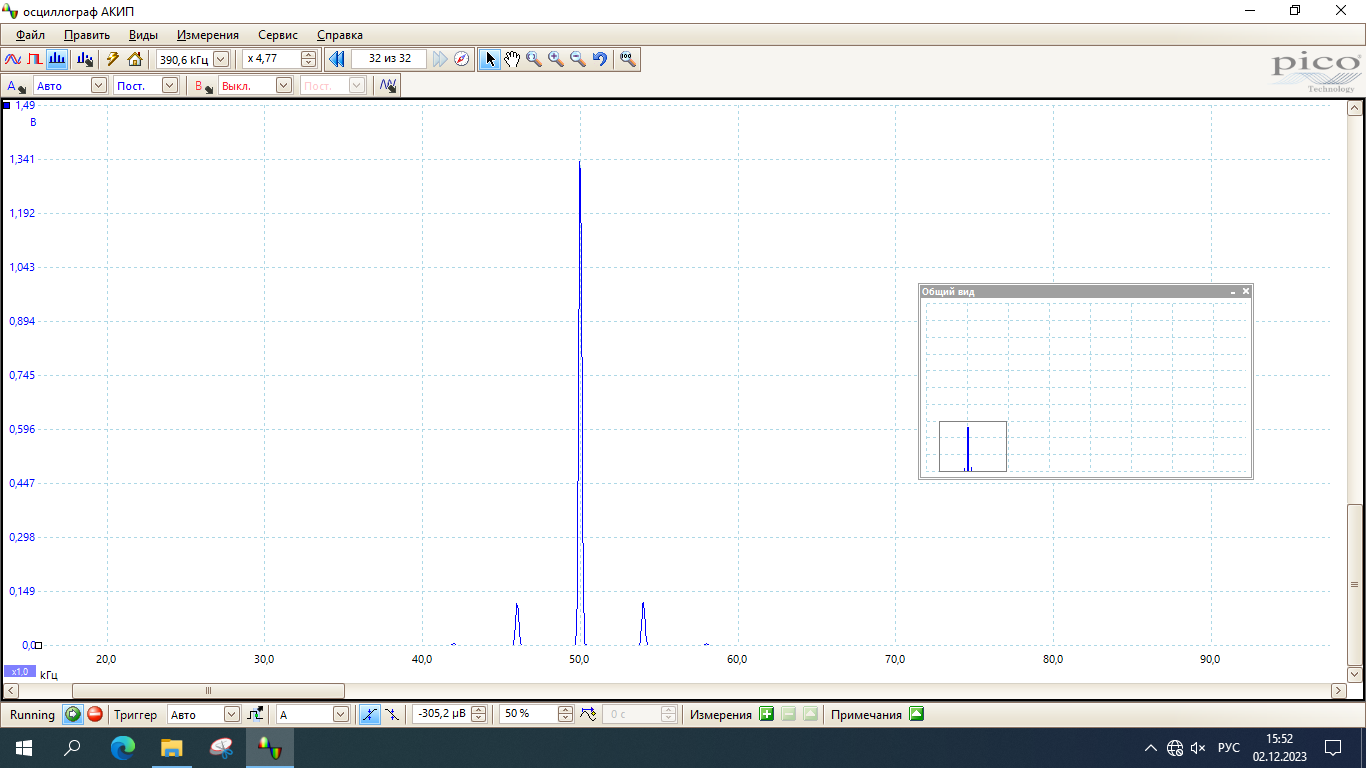
\includegraphics[width=1\linewidth]{D_50k_4k_10f.png}} $\nu_0$ = 50 кГц, $\nu_\text{мод}$ = 4 кГц, $\varphi$ = 10$\degree$  \\
\end{minipage}
\vfill
\caption{}
\label{ris:experimentalcorrelationsignals}
\end{figure}




\begin{figure}[h]
\begin{minipage}[h]{0.44\linewidth}
\center{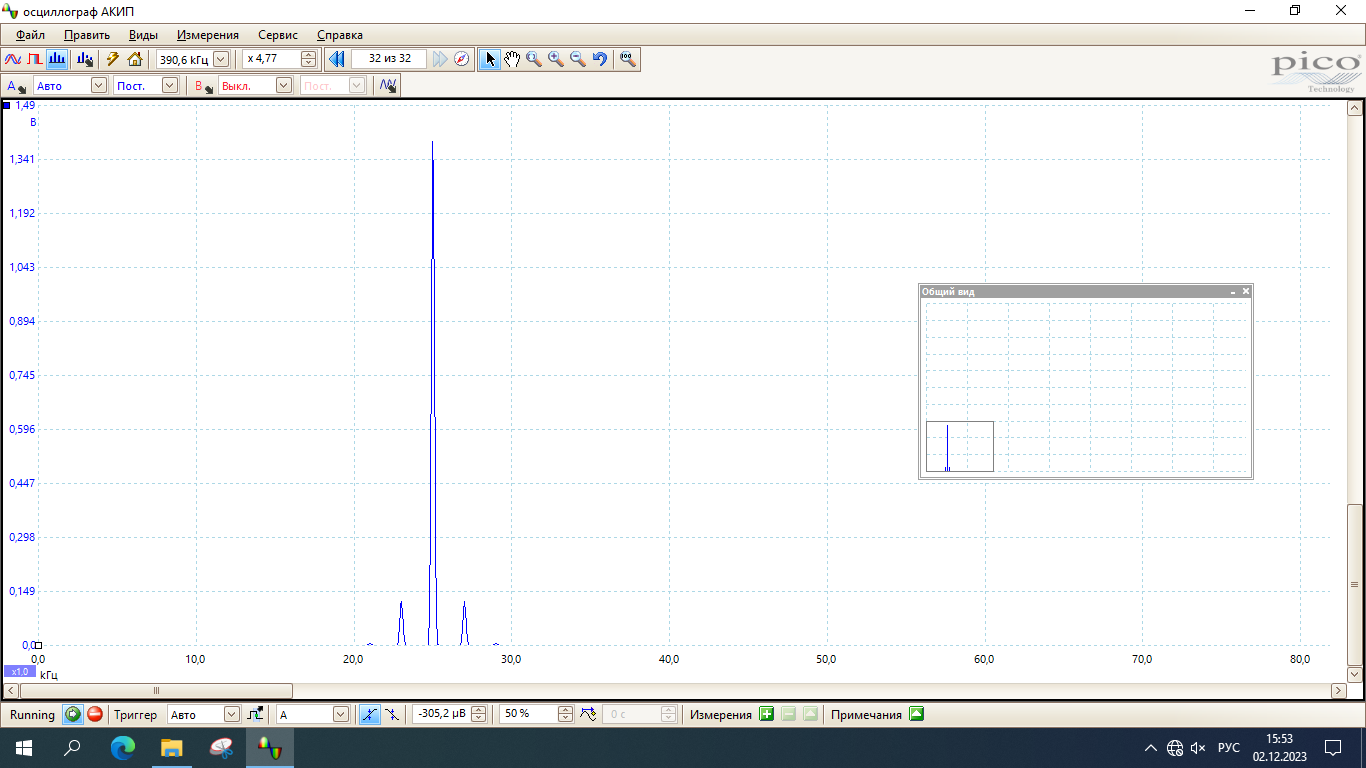
\includegraphics[width=1\linewidth]{D_25k_2k_10f.png}} $\nu_0$ = 25 кГц, $\nu_\text{мод}$ = 2 кГц, $\varphi$ = 10$\degree$  \\
\end{minipage}
\label{ris:experimentalcorrelationsignals}
\end{figure}




\end{enumerate}


\newpage










\subsection*{Е. Изучение фильтрации сигналов}



\begin{enumerate}
Подадим на вход RC-цепочки последовательность прямоугольных импульсов с периодом повторения $T = 3$ мкс и длительностью $\tau = 150$ нс. Получим спектр, представленный на рис. \ref{fig:RC}.

При том же фиксированном периоде $T$ проведем измерения отношения амплитуд соответствующих спектральных гармоник фильтрованного и исходного сигналов $K_n = \frac{|a^\phi_n}{a^0_n}$. Полученные данные представлены в таблице \ref{tab:RC}. Частоту можно почитать по формуле $\nu = \nu_0 n = n/T$.

При больших значениях частот K линейна. Построим её и по углу наклона определим $\tau_{RC}$

\begin{equation*}
    K(1/\nu) = \frac{1}{2\pi \tau_{RC}} \left(\frac{1}{\nu}\right)
\end{equation*}

Построим график $K(1\nu)$.

\begin{table}[h!]
    \centering
    \begin{tabular}{|c|c|c|c|c|c|c|}
    \hline
        $1/\num, \text{ кГц}^{-1}$ & 1.000 & 0.500 & 0.333 & 0.250 & 0.200 & 0.167  \\ \hline
        $K_n$ & 0.380 & 0.190 & 0.120 & 0.071 & 0.078 &  0.042 \\ \hline
    \end{tabular}
    \caption{Отношение амплитуд спектральных гармоник фильтрованного и исходного сигналов}
    \label{tab:RC}
\end{table}
\end{enumerate}

 Из коэффициента наклона получаем

 \begin{equation*}
     \tau_{RC} = (3.3 \pm 0.2)мкс
 \end{equation*}

\begin{figure}[h!]
    \centering
    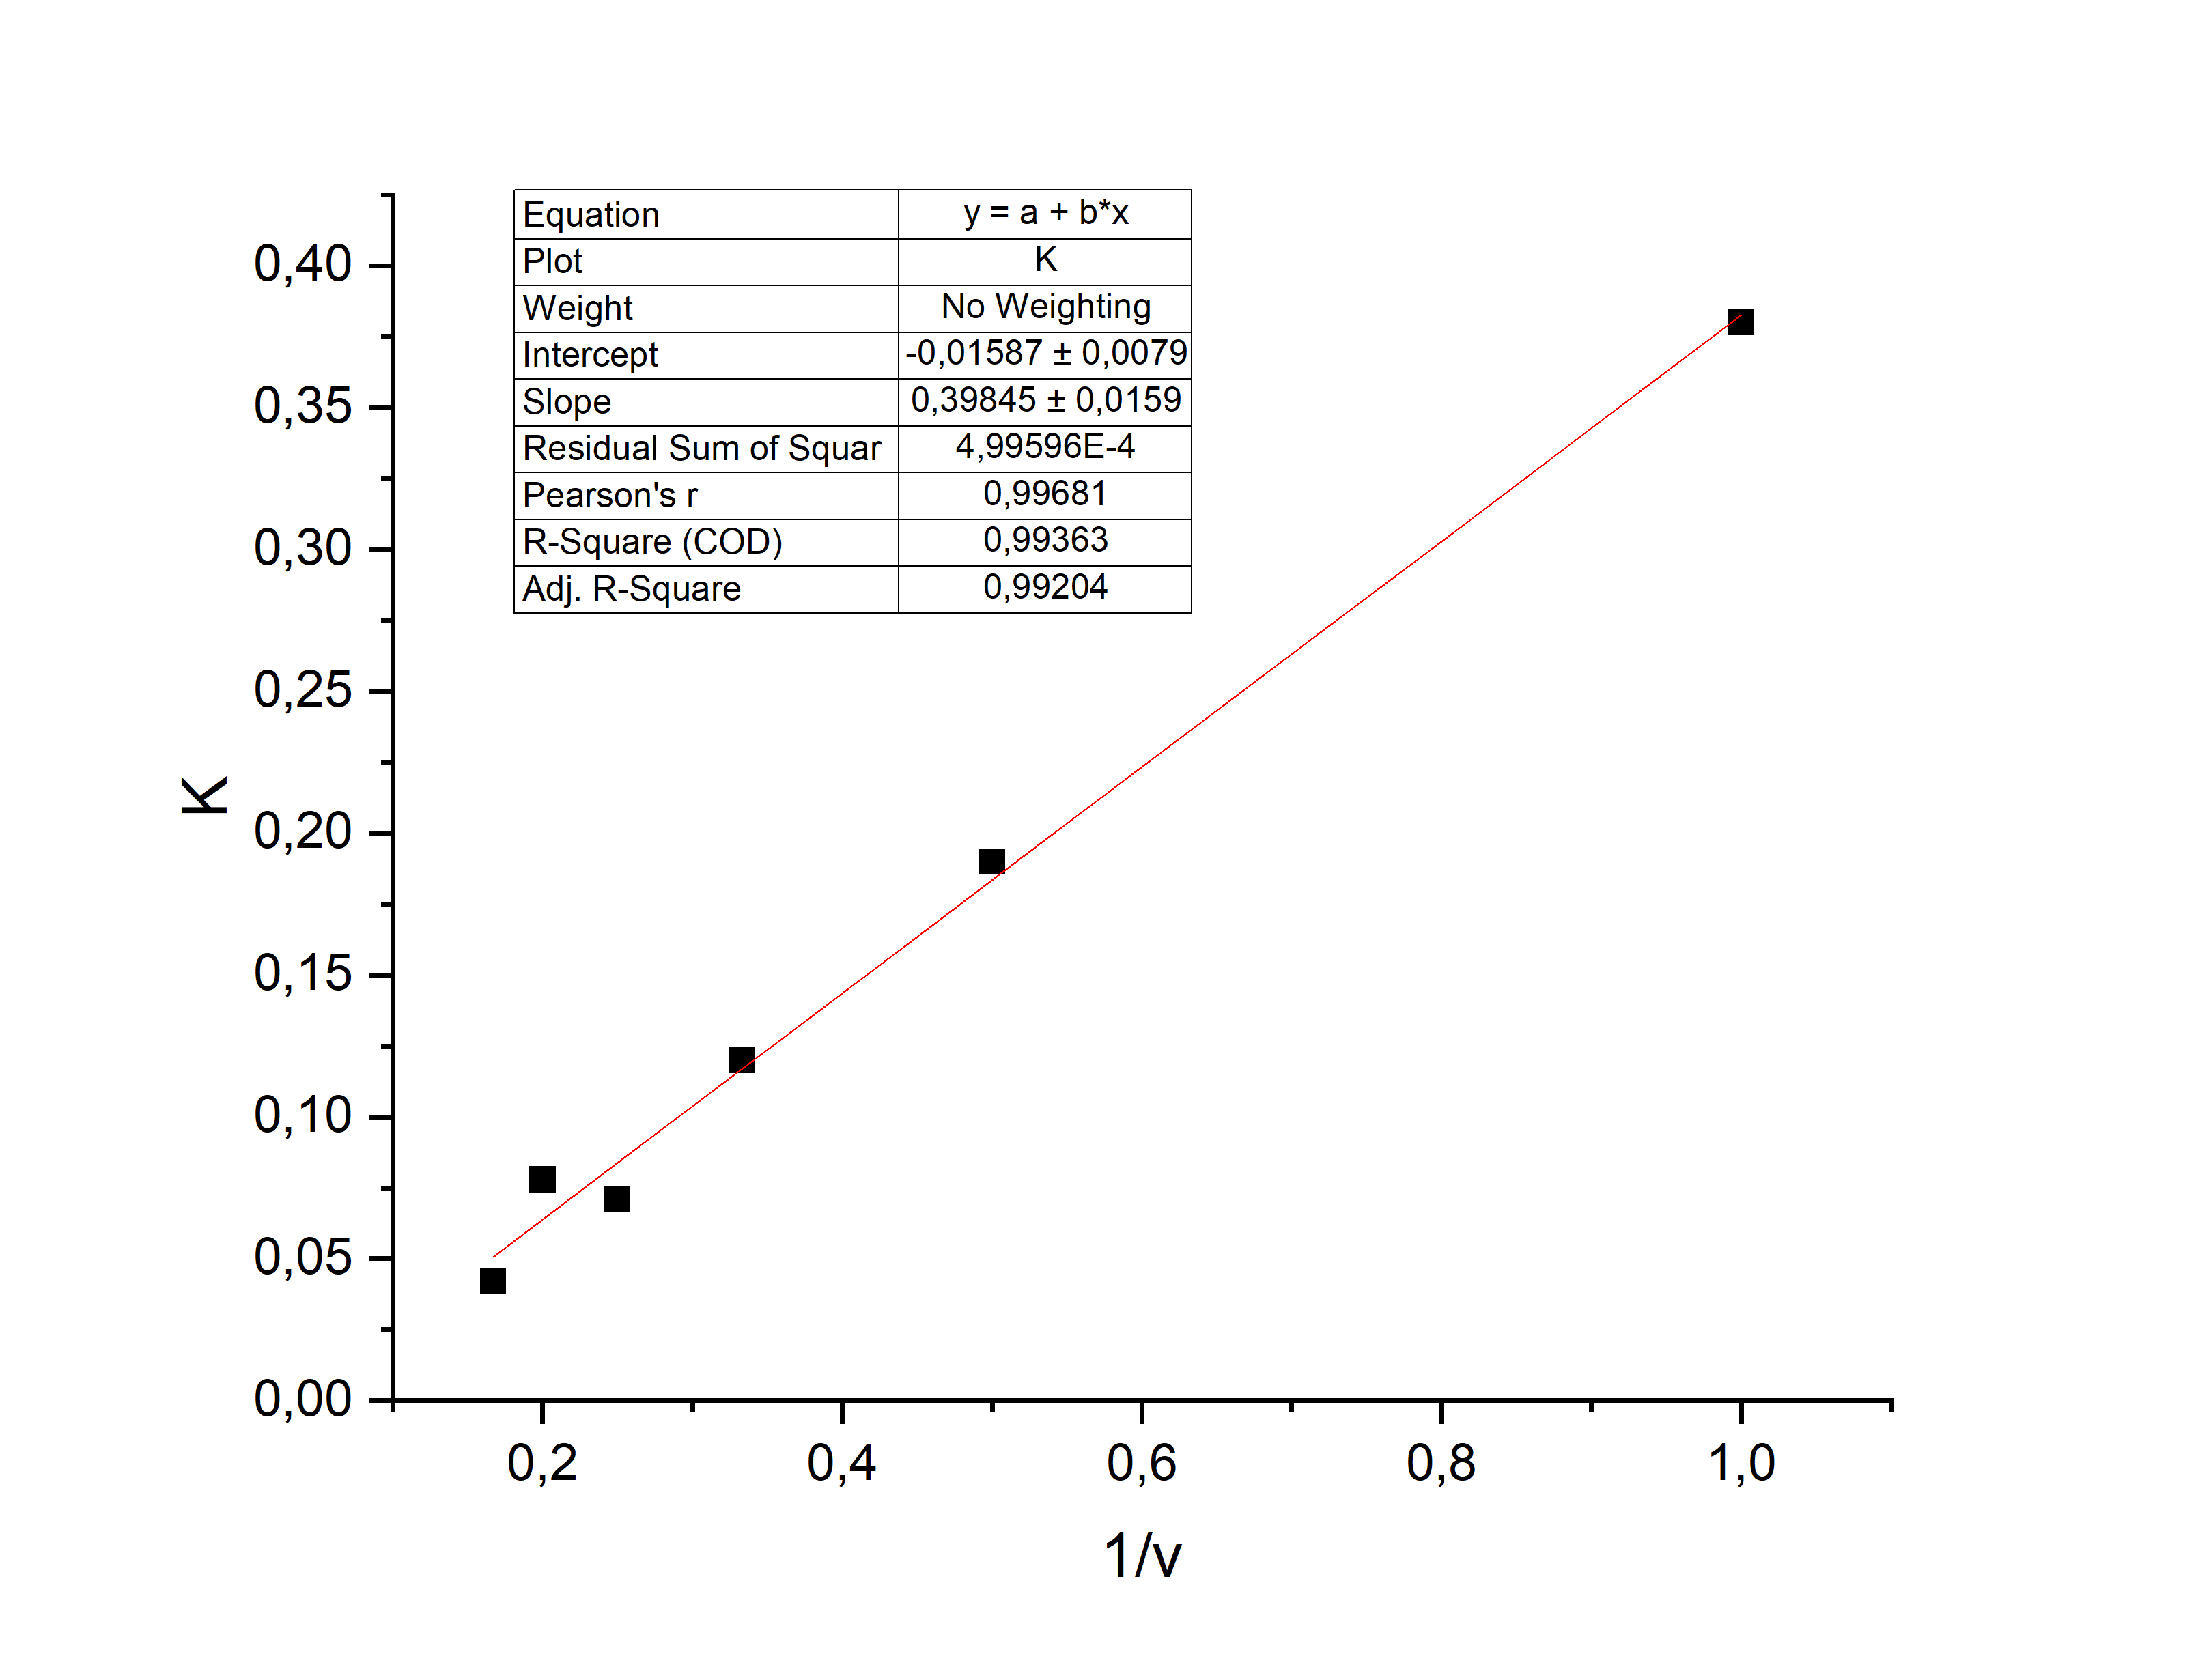
\includegraphics[width=15cm]{grafic4.png}
    \caption{Зависимость K от $\frac{1}{\nu}$}
    \label{fig:RC}
\end{figure}




\newpage



\section{Обсуждение результатов и выводы}

В данной работе мы изучили понятие спектра и спектрального анализа, исследовали спектральный состав периодических электрических сигналов, а также проанализировали фильтрацию сигналов при прохождении их через $RC$ контур. Проверили частный случай выполнения соотношения неопределённости.


\end{document}
